%=======================================================================
%
% ------------------------------------------------------------------------
% ------------------------------------------------------------------------
% abnTeX2: Modelo de Trabalho Academico  em conformidade com 
% ABNT NBR 14724:2011: Informacao e documentacao - Trabalhos academicos
% ------------------------------------------------------------------------
%Customização IFC
% ------------------------------------------------------------------------
% Autor:  Tiago Possato (tiago.possato@yahoo.com.br), baseado no modelo de Eliton Tiago (elitontiago@hotmail.com)
% Adaptação: Fábio Pinheiro (fabio.pinheiro@ifc.edu.br) e Henrique Pieri de Lima (henrique070425@gmail.com)
% Versão: maio de 2026
% Codificação: UTF-8
% LaTeX:  abnTeX2
%
%=======================================================================

\documentclass[
	% -- opções da classe memoir --
	12pt,				% tamanho da fonte	
	oneside,          % não imprimir em verso e anverso, oposto do twoside 
	a4paper,			% tamanho do papel. 
	% -- opções da classe abntex2 --
	chapter=TITLE,		% títulos de capítulos convertidos em letras maiúsculas
	section=TITLE,		% títulos de seções convertidos em letras maiúsculas
	subsection=TITLE,	% títulos de subseções convertidos em letras maiúsculas
	%subsubsection=TITLE,% títulos de subsubseções convertidos em letras maiúsculas
	% -- opções do pacote babel --
	english,			% idioma adicional para hifenização
	brazil			% o último idioma é o principal do documento
	,sumario=tradicional,
	]{abntex2-IFC}


% ---
% Pacotes fundamentais 
% ---
\usepackage{cmap}				% Mapear caracteres especiais no PDF
\usepackage{times}			    % Usa a fonte Times
\usepackage[T1]{fontenc}		% Selecao de codigos de fonte.fontenc
\usepackage[utf8]{inputenc}		% Codificacao do documento (conversão automática dos acentos)
\usepackage{lastpage}			% Usado pela Ficha catalográfica
\usepackage{indentfirst}		% Indenta o primeiro parágrafo de cada seção.
\usepackage{color}				% Controle das cores
\usepackage{graphicx}			% Inclusão de gráficos
\usepackage{amsfonts}			% Símbolos
%----Ajuste no alinhamento das listas
\usepackage{enumitem}
\setitemize[0]{itemindent=0.4cm,itemsep=0pt}
\setenumerate[0]{itemindent=0.5cm,itemsep=0pt}
%------
% ---
% Pacotes de citações
% ---
\usepackage[brazilian,hyperpageref]{backref}	 					  % Paginas com as citações na bibl

\usepackage[a4paper]{geometry}
%Referência
\usepackage[alf, 	
			 		abnt-emphasize=bf,
				    abnt-url-package=none,
				    abnt-repeated-title-omit=yes,
				    abnt-full-initials=yes,                                        %yes nome por extenso, no apenas iniciais
					abnt-etal-list=3												%abreviar com mais de 3 autores
]{abntex2/abntex2cite}				 														    % Citações padrão ABNT
\usepackage{lipsum}							   								       % para geração de dummy text
\usepackage{multirow}
\usepackage{float}
\usepackage{setspace}
\usepackage{tabularx}
\usepackage[table,xcdraw]{xcolor}
\usepackage{booktabs}			% \toprule, \midrule e \bottomrule usados nas tabelas do modelo
\usepackage{longtable}
\usepackage{array}
\newcolumntype{L}[1]{>{\raggedright\arraybackslash}p{#1}}

% --- Figuras e gráficos vetoriais
\usepackage{tikz}
\usetikzlibrary{positioning,arrows.meta,shapes.geometric,shapes.multipart,fit,backgrounds,calc,shadows}
\usepackage{pgfplots}
\pgfplotsset{compat=1.18, /pgf/number format/use comma, /pgf/number format/1000 sep={.}}
\renewcommand{\arraystretch}{1.2}

\tikzset{
  caixa/.style={draw, rounded corners=2pt, align=center, font=\footnotesize, minimum height=0.9cm, inner sep=4pt, fill=white},
  ia/.style={caixa, fill=black!8},
  ext/.style={caixa, dashed},
  seta/.style={-{Stealth[length=2.2mm]}, thick},
  grupo/.style={draw, rounded corners=4pt, inner sep=8pt, dashed, black!60},
  rotulo/.style={font=\scriptsize\itshape, align=center}
}

% --- Código-fonte nos apêndices
\usepackage{listings}
\lstdefinelanguage{JavaScript}{
  keywords={const,let,var,function,return,if,else,for,of,new,true,false,null,typeof,throw,try,catch},
  sensitive=true,
  comment=[l]{//},
  morecomment=[s]{/*}{*/},
  morestring=[b]',
  morestring=[b]",
  morestring=[b]`
}
\lstset{
  basicstyle=\ttfamily\scriptsize,
  breaklines=true,
  columns=fullflexible,
  keepspaces=true,
  frame=single,
  numbers=left,
  numberstyle=\tiny,
  showstringspaces=false,
  keywordstyle=\bfseries,
  commentstyle=\itshape\color{black!60},
  literate={á}{{\'a}}1 {à}{{\`a}}1 {ã}{{\~a}}1 {â}{{\^a}}1 {é}{{\'e}}1 {ê}{{\^e}}1 {í}{{\'i}}1
           {ó}{{\'o}}1 {õ}{{\~o}}1 {ô}{{\^o}}1 {ú}{{\'u}}1 {ç}{{\c c}}1 {Á}{{\'A}}1 {É}{{\'E}}1
           {Í}{{\'I}}1 {Ó}{{\'O}}1 {Ú}{{\'U}}1 {Ç}{{\c C}}1 {Ã}{{\~A}}1 {—}{{---}}1 {–}{{--}}1
           {⚙}{{}}0 {·}{{$\cdot$}}1 {Õ}{{\~O}}1 {Ê}{{\^E}}1 {️}{{}}0 {→}{{$\rightarrow$}}1
}
%\usepackage[none]{hyphenat}
%\captionsetup[table]{justification=raggedright}
% Configurações de aparência do PDF final
% alterando o aspecto da cor azul
\definecolor{blue}{RGB}{41,5,195}

% --- 
% Espaçamentos entre linhas e parágrafos 
% --- 
% O tamanho do parágrafo é dado por:
\setlength{\parindent}{2cm}
\linespread{1.5}

%Espaçamento depois dos títulos
\setlength{\afterchapskip}{\baselineskip}
% %\setlength{\afterchapskip}{\lineskip}

% Controle do espaçamento entre um parágrafo e outro:
\setlength{\parskip}{0cm}  % tente também \onelineskip
\setlength{\emergencystretch}{2em} % evita linhas além da margem em parágrafos com termos longos

\hangcaption
\captionstyle[\raggedright]{}

%Estava mostrando nas referencias quais paginas estavam sendo referenciadas
\renewcommand{\backref}{}
\renewcommand*{\backrefalt}[4]{}

%Reduzir a fonte do caption
%\captionnamefont{\centering\ABNTEXfontereduzida}
%\captiontitlefont{\centering\ABNTEXfontereduzida}
%Ajuste nas listas de tabela, ilustrações e quadros
\setlength\cftbeforechapterskip{0pt}
% ---
% compila o indice
% ---
\makeindex
% ---

%----Include da capa é fora do documento 
% ---
% Informações de dados para CAPA e FOLHA DE ROSTO
% ---

\titulo{\uppercase{Sistema de suporte à validação de planos de ensino com modelos de linguagem: um estudo de caso no curso de Ciência da Computação do IFC -- Campus Videira}}
\autor{\uppercase{Vinícius Slongo}}
\local{Videira}
\data{2026}
\orientador[Orientador:]{Prof. Me. Fabricio Bizotto}
\instituicao{ Ministério da Educação\\
        Secretaria de Educação Profissional e Tecnológica\\
        Instituto Federal Catarinense\\
        Campus Videira}
\tipotrabalho{Trabalho de Conclusão de Curso}
% O preambulo deve conter o tipo do trabalho, o objetivo,
% o nome da instituição e a área de concentração
\preambulo{Trabalho de Conclusão de Curso apresentado ao
Curso de graduação em Ciência da Computação do
Instituto Federal Catarinense -- Campus Videira para
obtenção do título de bacharel em Ciência da Computação.

Orientador: \imprimirorientador}
% ---

%---

\begin{document}
% Retira espaço extra obsoleto entre as frases.
\frenchspacing 

% ----------------------------------------------------------
% ELEMENTOS PRÉ-TEXTUAIS
% ----------------------------------------------------------

%--- CAPA ----
\imprimircapa

% --- FOLHA DE ROSTO
\imprimirfolhaderosto
% \imprimirfolhaderosto* (o * indica que haverá a ficha bibliográfica)

% Inserir FOLHA DE APROVAÇÃO
\begin{folhadeaprovacao}

  \begin{center}
  \vspace*{-1.2cm}
    \textbf{\large\imprimirautor}

    \vspace*{\fill}\vspace*{\fill}\vspace*{\fill}
    \parbox{15cm}{
        \OnehalfSpacing\centering\large\textbf{\imprimirtitulo}
    }
    \vspace*{\fill}\vspace*{\fill}

    \hspace{.45\textwidth}
    \begin{minipage}{.5\textwidth}
        Este Trabalho de Curso foi julgado
        adequado para a obtenção do título de
        Bacharel em Ciência da Computação e
        aprovado em sua forma final pelo curso de
        graduação em Ciência da Computação do Instituto Federal Catarinense
        -- Campus Videira.
    \end{minipage}%
    \vspace*{\fill}
   \end{center}
    \vspace{-1cm}
  \begin{center}
  	 % Preencher com a data da defesa
  	 Videira (SC), \rule{1cm}{0.4pt} de \rule{3cm}{0.4pt} de 2026
  \end{center}

   \assinatura{\begin{center}\vspace{-0.7cm}\imprimirorientador \\
   					   Instituto Federal Catarinense -- Campus Videira
   					   \end{center}
   			  }

    \begin{center}
  	\textbf{BANCA EXAMINADORA}
   \end{center}
   % Preencher com titulação e nome dos membros da banca (ex.: Prof. Dr. João da Silva)
   \assinatura{\begin{center}\vspace{-0.7cm}Prof.(ª) Titulação Nome do(a) avaliador(a) 1\\
   					   Instituto Federal Catarinense -- Campus Videira
   					     \end{center}
   }
    \assinatura{\begin{center}\vspace{-0.7cm}Prof.(ª) Titulação Nome do(a) avaliador(a) 2\\
   					    Instituto Federal Catarinense -- Campus Videira
   					    \end{center}
    }

    \vspace*{1cm}

\end{folhadeaprovacao}


% Inserir FOLHA DE AUTORIZAÇÃO (preencher matrícula e CPF antes de ativar)
% \begin{folhadeautorizacao}

  \begin{center}
  \vspace*{1 cm}
  \vspace{-2cm}
   \centering
\includegraphics[width=1.5cm]{brasaoRepublicaPeB.jpg}
   \vspace{-0.5 cm}
    {\large \SingleSpacing \imprimirinstituicao}
    \vspace{-0.5cm}
    \center{ \hrulefill}
    
     {\large \SingleSpacing \textbf{Autorização}}
    
    
    \vspace*{1 cm}
    
    \raggedleft{ Videira (SC), 19 de Novembro de 2016}
    \vspace*{0.5 cm}
    
   \end{center}
   


Eu, NOME SOBRENOME, regularmente matriculado na disciplina de Trabalho de Conclusão de Curso II - TC II do curso de Bacharel em Ciência da Computação, sob matrícula nº. XXXXXXX, pelo presente documento, autorizo o Instituto Federal Catarinense - IFC-Câmpus Videira, a utilizar o meu TC II intitulado "\imprimirtitulo", sob a orientação d Professor \imprimirorientador, para futuras informações e divulgações promovidas pelo Curso, e pelo Instituto, de forma institucional, em todo território nacional e internacional, sem fins comerciais, por qualquer meio de comunicação, tornando-o acessível a qualquer pessoa com interesse no trabalho.

A presente autorização substancia um consentimento de vontade e isenta de qualquer vício, feito de forma gratuita, e no gozo da minha capacidade civil, pelo que declaro nada me ser devido pelo curso de Ciência da Computação e pelo IFC-Câmpus Videira, ou seus representantes, em tempo algum, seja que título for, no que se refere, direta ou indiretamente, ao presente consentimento de uso da minha imagem e meu trabalho.

Declaro, ainda, que a utilização de meu nome e de meu trabalho, não constitui ofensa ou violação de meus direitos, nos termos do inciso X, do artigo 5o. da Constituição Federal.

Pelo presente também declaro ser de minha total responsabilidade o conteúdo de meu trabalho de conclusão de curso, descrito neste documento.

Os direitos e as obrigações aqui avençados transmitem-se aos meus herdeiros e sucessores.



  
   
   \vspace*{\fill}
   \vspace{-0.5 cm}
   
   \noindent Nome: \imprimirautor
   
   \vspace{0.25 cm}
   
   \noindent CPF: XXXXXXXXXXXXXX
   
   \vspace{0.25 cm}
   
   \noindent Assinatura: \hskip-3em\vtop{\vskip.05cm\hsize=5in \hrulefill}
   
   \vspace{0.5 cm}
   
    \begin{center}
    Rod. SC 135, KM 125 - Campo Experimental - CEP: 89560-000 - Videira - SC \\
    Fone: (49) 3533-4900 - http://www.ifc-videira.edu.br
    \end{center}

    \vspace*{1cm}
  
\end{folhadeautorizacao}

% DEDICATÓRIA
\begin{dedicatoria}
 \vspace*{\fill}
 \noindent
  \raggedleft
 \begin{minipage}{.54\textwidth}
    % Texto-base: personalize antes da entrega.
    Dedico este trabalho à minha família, que sempre acreditou na educação como caminho.
   \end{minipage}
\end{dedicatoria}


% AGRADECIMENTO
\begin{agradecimentos}

% Texto-base: personalize com nomes e situações reais antes da entrega.
Agradeço, em primeiro lugar, à minha família, pelo apoio e pela paciência ao longo de toda a graduação.

Ao professor Fabricio Bizotto, pela orientação, pela disponibilidade e pelas sugestões que deram forma aos critérios de avaliação adotados neste trabalho.

Aos professores e servidores do Instituto Federal Catarinense -- Campus Videira, pela formação recebida e pelo acesso aos planos de ensino que tornaram possível a avaliação do sistema.

Aos colegas de curso, pela convivência e pela troca de conhecimento durante esses anos.

\end{agradecimentos}


%EPÍGRAFE
\begin{epigrafe}
    \vspace*{\fill}
    \begin{flushright}
        \begin{minipage}{.6\textwidth}
        \raggedleft
        \textit{Ensinar não é transferir conhecimento, mas criar as possibilidades para a sua própria produção ou a sua construção.}\\[0.3cm]
        Paulo Freire, \textit{Pedagogia da autonomia}
        \end{minipage}
    \end{flushright}
\end{epigrafe}


% RESUMO
% resumo em português
\begin{resumo}
\noindent
No Instituto Federal Catarinense (IFC), cada componente curricular possui um plano de ensino que deve conter os elementos exigidos pela Organização Didática da instituição, e a conferência desses documentos é feita manualmente pela coordenação e pelo Núcleo Docente Estruturante (NDE), tarefa repetitiva e sujeita a inconsistências entre avaliadores. Este trabalho apresenta o desenvolvimento e a avaliação de um sistema semiautomático de apoio à validação de planos de ensino do curso de Ciência da Computação do IFC -- Campus Videira. A solução, construída sobre a plataforma de automação n8n e executada em contêineres Docker, obtém os planos em PDF de uma pasta do Google Drive, extrai e segmenta o texto em seções, avalia doze critérios com um modelo de linguagem de grande escala (LLM) aberto, o Qwen2.5 de 7 bilhões de parâmetros executado localmente pelo Ollama, e registra o resultado de cada critério (OK, INCOMPLETO ou AUSENTE) em uma planilha consultada por um painel \textit{web}. Para reduzir alucinações, a arquitetura combina o LLM com saída estruturada por esquema JSON e com regras determinísticas, como a contagem de referências bibliográficas por expressões regulares. O desenvolvimento seguiu um processo iterativo e incremental, e a avaliação usou os 29 planos de ensino do semestre 2024/1. Ao longo das iterações, a proporção de planos com falha técnica caiu de 86,2\% para zero, e a versão final processou o lote completo em 8 minutos e 54 segundos, com média de 11,5 segundos de inferência por plano em uma GPU de 6 GB. Na execução final, 11 planos (38\%) foram considerados conformes, 3 (10\%) pendentes e 15 (52\%) reprovados, e a ausência do horário de atendimento ao estudante foi a não conformidade mais frequente. No critério verificável por oráculo estrutural, o sistema obteve \textit{recall} de 100\%, precisão de 93,8\% e Kappa de Cohen de 0,93. A análise de erros identificou limitações, como textos provisórios do sistema acadêmico aceitos como conteúdo válido e observações gerais do modelo contraditórias com o resultado por critério, que orientam os trabalhos futuros. Conclui-se que o sistema é viável como ferramenta de triagem que reduz o esforço de conferência, desde que a decisão final permaneça com o avaliador humano.

 \vspace{0.2cm}
\noindent Palavras-chave: Inteligência artificial. Modelos de linguagem. Plano de ensino. Automação de processos. n8n.

\end{resumo}

% resumo em inglês
\begin{resumo}[Abstract]
\begin{otherlanguage*}{english}
\noindent
At the Instituto Federal Catarinense (IFC), every course unit has a teaching plan that must contain the elements required by the institution's academic regulations, and these documents are checked manually by the program coordination and the Structuring Teaching Nucleus (NDE), a repetitive task prone to inconsistencies between reviewers. This work presents the development and evaluation of a semi-automatic system that supports the validation of teaching plans in the Computer Science program at IFC -- Videira Campus. The solution, built on the n8n automation platform and deployed with Docker containers, retrieves the plans as PDF files from a Google Drive folder, extracts and segments their text into sections, assesses twelve criteria with an open large language model (LLM), the 7-billion-parameter Qwen2.5 running locally on Ollama, and stores the result of each criterion (OK, INCOMPLETE or MISSING) in a spreadsheet displayed by a web dashboard. To reduce hallucinations, the architecture combines the LLM with JSON-schema structured output and with deterministic rules, such as counting bibliographic references with regular expressions. Development followed an iterative and incremental process, and the evaluation used the 29 teaching plans of the 2024/1 semester. Across iterations, the share of plans with technical failures dropped from 86.2\% to zero, and the final version processed the whole batch in 8 minutes and 54 seconds, averaging 11.5 seconds of inference per plan on a 6 GB GPU. In the final run, 11 plans (38\%) were compliant, 3 (10\%) pending and 15 (52\%) rejected, and the missing student office hours was the most frequent non-compliance. On the criterion that could be checked by a structural oracle, the system reached 100\% recall, 93.8\% precision and a Cohen's Kappa of 0.93. The error analysis revealed limitations, such as placeholder texts from the academic system being accepted as valid content and general remarks from the model contradicting the per-criterion results, which guide future work. The system proved viable as a screening tool that reduces review effort, provided that the final decision remains with the human reviewer.

\vspace{0.2cm}
\noindent Keywords: Artificial intelligence. Language models. Teaching plan. Process automation. n8n.
\end{otherlanguage*}
\end{resumo}


% lista de ilustrações
\pdfbookmark[0]{\listfigurename}{lof}
\listoffigures*
\cleardoublepage
% ---

% lista de quadros
% --- 
%PRECISO VER COMO FAZER O CONTROLE DE QUANDO TIVER MENOS Q 10 VAI PARA LISTA DE ILUSTRAÇÕES
\pdfbookmark[0]{\listofquadrosname}{loq}
%\listofquadros*
%\cleardoublepage
% ---

% LISTA DE TABELAS
\pdfbookmark[0]{\listtablename}{lot}
\listoftables*
\cleardoublepage

% ---
% inserir lista de abreviaturas e siglas
% ---
\begin{siglas}
  \item[API] \textit{Application Programming Interface} (Interface de Programação de Aplicações)
  \item[CCO] Curso de Ciência da Computação
  \item[CPU] \textit{Central Processing Unit} (Unidade Central de Processamento)
  \item[FN] Falso negativo
  \item[FP] Falso positivo
  \item[GPU] \textit{Graphics Processing Unit} (Unidade de Processamento Gráfico)
  \item[HTML] \textit{HyperText Markup Language}
  \item[HTTP] \textit{Hypertext Transfer Protocol}
  \item[IA] Inteligência Artificial
  \item[IFC] Instituto Federal Catarinense
  \item[JSON] \textit{JavaScript Object Notation}
  \item[KV] \textit{Key-Value} (cache de chaves e valores da atenção)
  \item[LDB] Lei de Diretrizes e Bases da Educação Nacional
  \item[LGPD] Lei Geral de Proteção de Dados Pessoais
  \item[LLM] \textit{Large Language Model} (Modelo de Linguagem de Grande Escala)
  \item[MLOps] \textit{Machine Learning Operations}
  \item[NDE] Núcleo Docente Estruturante
  \item[OAuth] \textit{Open Authorization}
  \item[PDF] \textit{Portable Document Format}
  \item[PLN] Processamento de Linguagem Natural
  \item[PPC] Projeto Pedagógico de Curso
  \item[RAG] \textit{Retrieval-Augmented Generation} (Geração Aumentada por Recuperação)
  \item[RF] Requisito Funcional
  \item[RN] Regra de Negócio
  \item[RNF] Requisito Não Funcional
  \item[SIGAA] Sistema Integrado de Gestão de Atividades Acadêmicas
  \item[UML] \textit{Unified Modeling Language}
  \item[VN] Verdadeiro negativo
  \item[VP] Verdadeiro positivo
  \item[VRAM] \textit{Video Random Access Memory}
\end{siglas}
% ---

% ---
% inserir lista de símbolos
% ---
%\begin{simbolos}
%  \item[$ \Gamma $] Descrever o que o símbolo representa em seu trabalho. Exemplo abaixo.
%  \item[$ \omega $] Frequência angular [rad/s].
%  \item[$ \zeta $] Coeficiente de amortecimento.

%\end{simbolos}
% ---

% SUMARIO
\pdfbookmark[0]{\contentsname}{toc}
\tableofcontents*
\cleardoublepage

% ------------------------------------------------------
% ELEMENTOS TEXTUAIS
% ------------------------------------------------------
\textual
% INTRODUÇÃO
\chapter{INTRODUÇÃO}
\label{cap:introducao}

Os avanços recentes em Inteligência Artificial (IA), em especial no Processamento de Linguagem Natural (PLN) e nos modelos de linguagem de grande escala (\textit{Large Language Models}, LLMs), ampliaram as possibilidades de automação de tarefas que antes dependiam exclusivamente da leitura humana de documentos \cite{Zhao2023, ADIGUZEL2023}. A UNESCO aponta que a IA pode apoiar tanto a aprendizagem quanto a gestão educacional, desde que sua adoção seja acompanhada de políticas que garantam equidade e supervisão humana \cite{Pedro2019}. No Brasil, pesquisa da Chegg.org divulgada pela \citeonline{CNNBrasil2023} indica que cerca de metade dos universitários já utiliza ferramentas de IA em sua rotina acadêmica, o que evidencia a rápida difusão dessas tecnologias no ambiente educacional.

No campo da gestão educacional, \citeonline{Sposato2025} classifica as aplicações de IA na liderança e na administração de instituições de ensino e destaca a automação de tarefas rotineiras, a análise de documentos e o suporte à tomada de decisão como usos recorrentes. A revisão sistemática de \citeonline{Tan2025} reforça esse cenário ao identificar o apoio ao planejamento docente e a otimização de tarefas administrativas entre as aplicações mais frequentes, ao mesmo tempo em que aponta a escassez de estudos sobre processos administrativos do ensino superior. \citeonline{Walter2024}, por sua vez, ressalta que a integração da IA na educação exige letramento em IA e pensamento crítico, o que reforça a necessidade de manter a supervisão humana em qualquer solução automatizada.

Entre os documentos que estruturam o trabalho docente está o plano de ensino. A Lei de Diretrizes e Bases da Educação Nacional (LDB) atribui aos docentes a incumbência de elaborar e cumprir seu plano de trabalho e determina que as instituições informem aos estudantes, antes de cada período letivo, os programas dos componentes curriculares e seus critérios de avaliação \cite{Brasil1996}. No Instituto Federal Catarinense (IFC), cada componente curricular possui um plano de ensino elaborado pelo docente a cada semestre, e a Organização Didática da instituição define os elementos que esse documento deve conter, como ementa, objetivos, conteúdos, metodologia, avaliação e referências bibliográficas \cite{ifc2022}. A verificação de que cada plano contém esses elementos é feita manualmente pela coordenação de curso e pelo Núcleo Docente Estruturante (NDE), lendo documento por documento.

Essa conferência manual é repetitiva e sujeita a inconsistências entre avaliadores, e seu custo cresce com o número de componentes curriculares. Automatizá-la, contudo, não é trivial: os planos de ensino do IFC são emitidos pelo Sistema Integrado de Gestão de Atividades Acadêmicas (SIGAA) em um formato padronizado, com as mesmas seções em todos os documentos, mas o conteúdo de cada seção é texto livre e heterogêneo, escrito por docentes diferentes. Regras fixas conseguem verificar se uma seção existe ou quantas referências ela contém, mas não se uma metodologia descreve de fato como as aulas serão conduzidas. Esse tipo de julgamento exige interpretar o texto, tarefa para a qual os LLMs são adequados. Esses modelos, porém, estão sujeitos a alucinações, isto é, à geração de conteúdo plausível porém incorreto \cite{Ji2023}, de modo que, aplicados à conferência dos planos, seus apontamentos precisam ser verificáveis e a decisão sobre cada plano precisa permanecer com o avaliador humano \cite{USDeptEd2023, Shneiderman2022}.

Diante desse cenário, este trabalho propõe desenvolver um sistema semiautomático de apoio à validação dos planos de ensino do curso de Ciência da Computação do IFC -- Campus Videira e avaliá-lo com os planos reais de um semestre letivo. O sistema deverá obter os planos em PDF de uma pasta compartilhada, extrair e segmentar seu texto, avaliar doze critérios com um LLM aberto executado localmente, combinar essa avaliação com regras determinísticas e apresentar o resultado de cada critério em um painel \textit{web}, para que a coordenação e o NDE possam identificar os planos e os itens que exigem revisão. A avaliação busca verificar se essa abordagem é tecnicamente viável em um equipamento local e em que medida seus apontamentos concordam com verificações de referência.

\section{Problema de pesquisa}

De que forma um sistema baseado em modelos de linguagem pode apoiar a verificação da conformidade dos planos de ensino às normas do IFC, indicando de forma confiável os itens que exigem revisão e preservando o controle humano sobre a decisão final?

\section{Objetivos}

Para responder ao problema de pesquisa, foram definidos um objetivo geral e quatro objetivos específicos, apresentados a seguir.

\subsection{Objetivo Geral}

Desenvolver e avaliar um sistema semiautomático baseado em IA para apoiar a validação dos planos de ensino do curso de Ciência da Computação do IFC -- Campus Videira, alinhado à Organização Didática da instituição.

\subsection{Objetivos Específicos}

\begin{itemize}
    \item Identificar os elementos obrigatórios dos planos de ensino a partir da Organização Didática do IFC e das orientações da coordenação do curso, convertendo-os em critérios de avaliação verificáveis.
    \item Projetar e implementar um \textit{pipeline} de automação que extraia e segmente o texto dos planos, avalie cada critério com um LLM executado localmente e registre os resultados de forma rastreável.
    \item Disponibilizar um painel \textit{web} que permita acompanhar os planos processados e consultar o resultado e a justificativa de cada critério.
    \item Avaliar o sistema com os 29 planos de ensino reais do semestre 2024/1, medindo a proporção de planos com falha técnica em cada iteração (robustez técnica), o tempo de inferência por plano e de processamento do lote (desempenho computacional) e a concordância dos resultados com um oráculo estrutural e com a conferência manual dos apontamentos no texto dos planos, e analisar os erros encontrados para propor aprimoramentos.
\end{itemize}

\section{Justificativa}

A conferência manual dos planos de ensino consome tempo da coordenação e do NDE que poderia ser dedicado a ações pedagógicas de maior impacto, como a análise da coerência entre componentes curriculares e a atualização do Projeto Pedagógico de Curso (PPC). Por ser repetitiva, essa conferência também está sujeita a variações entre avaliadores e entre semestres, o que dificulta garantir que todos os planos atendam aos mesmos critérios.

Do ponto de vista científico, a revisão de \citeonline{Vieira2025} sobre as experiências com IA nos Institutos Federais constatou pouca produção acadêmica sobre o tema e identificou a IA como apoio administrativo como a forma de incorporação menos explorada. A aplicação de LLMs à verificação normativa de documentos acadêmicos internos é, portanto, um nicho pouco investigado, especialmente em instituições públicas brasileiras e com modelos executados localmente.

Do ponto de vista prático, a opção por ferramentas de código aberto e por um modelo executado em equipamento próprio elimina custos de licenciamento e evita o envio dos documentos a serviços externos de IA, o que facilita a adoção institucional e o atendimento à Lei Geral de Proteção de Dados Pessoais (LGPD) \cite{Brasil2018}. Por fim, a abordagem semiautomática, em que o sistema aponta possíveis não conformidades e o avaliador humano decide, segue as recomendações de uso responsável de IA na educação \cite{USDeptEd2023, Pedro2019}.

\section{Estrutura do trabalho}

Além desta introdução, o trabalho está organizado em cinco capítulos. O Capítulo \ref{cap:fundamentacao} apresenta a fundamentação teórica sobre planos de ensino, modelos de linguagem, técnicas para reduzir alucinações, ferramentas de automação e métricas de avaliação, além dos trabalhos relacionados. O Capítulo \ref{cap:metodologia} descreve a metodologia da pesquisa, incluindo o corpus utilizado e o protocolo de avaliação. O Capítulo \ref{cap:desenvolvimento} documenta o desenvolvimento do sistema: requisitos, atores, regras de negócio, histórias de usuário, modelagem de dados, diagramas e protótipo. O Capítulo \ref{cap:resultados} apresenta e discute os resultados da avaliação. Por fim, o Capítulo \ref{cap:conclusao} apresenta as conclusões, as limitações e as sugestões de trabalhos futuros.


% FUNDAMENTAÇÃO TEÓRICA E TRABALHOS RELACIONADOS
\chapter{FUNDAMENTAÇÃO TEÓRICA}
\label{cap:fundamentacao}

Este capítulo apresenta os conceitos que sustentam o trabalho. A Seção \ref{sec:plano} discute o plano de ensino e as normas que regem sua elaboração no IFC. As Seções \ref{sec:llm} a \ref{sec:local} tratam dos modelos de linguagem, de suas limitações, das técnicas empregadas para torná-los confiáveis e de sua execução em equipamento local. A Seção \ref{sec:automacao} aborda as ferramentas de automação e infraestrutura, a Seção \ref{sec:humano} discute o papel do avaliador humano e a Seção \ref{sec:metricas} apresenta as métricas de avaliação utilizadas. Por fim, a Seção \ref{sec:relacionados} revisa os trabalhos relacionados.

\section{O plano de ensino e as normas institucionais}
\label{sec:plano}

O planejamento é uma atividade de reflexão e de organização da ação docente, por meio da qual o professor articula os objetivos, os conteúdos, os métodos e a avaliação de forma coerente com a proposta pedagógica da instituição \cite{Libaneo1994}. O plano de ensino é o registro desse planejamento para um componente curricular em um período letivo. Ele serve, ao mesmo tempo, como guia para o docente, como compromisso público com os estudantes e como instrumento de acompanhamento para a gestão do curso.

A LDB estabelece que os docentes devem elaborar e cumprir seu plano de trabalho segundo a proposta pedagógica do estabelecimento e que as instituições de educação superior devem informar aos interessados, antes de cada período letivo, os programas dos cursos e componentes curriculares, seus requisitos e seus critérios de avaliação \cite{Brasil1996}. No IFC, a Organização Didática dos Cursos detalha essas exigências e define os elementos que devem constar no plano de ensino, que é submetido à apreciação da coordenação e do NDE do curso \cite{ifc2022}.

Na prática do IFC, o plano de ensino é registrado no SIGAA e exportado como um documento PDF com estrutura padronizada: identificação do componente e do docente, ementa, metodologia, procedimentos de avaliação, horário de atendimento, objetivos, conteúdo programático, cronograma de aulas, avaliações previstas e referências básicas e complementares. Embora a ordem e os rótulos das seções sejam fixos, o conteúdo de cada seção é texto livre, escrito por docentes diferentes, com estilos, extensões e graus de detalhamento distintos. Essa combinação de estrutura fixa e conteúdo livre é o que motiva a abordagem híbrida adotada neste trabalho: regras determinísticas para o que é estrutural e modelos de linguagem para o que exige interpretação.

\section{Modelos de linguagem}
\label{sec:llm}

Como visto na seção anterior, o plano de ensino tem estrutura fixa, mas o conteúdo de cada seção é texto livre. Verificar se esse conteúdo atende às normas exige uma tecnologia capaz de interpretar linguagem natural, e a que fundamenta este trabalho são os modelos de linguagem. Eles são objeto de estudo do PLN, a área da IA que trata da compreensão e da geração de linguagem humana por computadores \cite{RussellNorvig2021, Jurafsky2025}.

Um modelo de linguagem atribui probabilidades a sequências de palavras e, de forma equivalente, estima a probabilidade da próxima unidade de texto (\textit{token}) dada a sequência anterior \cite{Jurafsky2025}. Os LLMs são modelos de linguagem com bilhões de parâmetros, treinados sobre grandes volumes de texto. Com o aumento de escala, esses modelos passaram a exibir a capacidade de executar tarefas novas apenas a partir de instruções e exemplos fornecidos na entrada, sem ajuste dos pesos, fenômeno conhecido como aprendizado em contexto (\textit{in-context learning}) \cite{Brown2020, Zhao2023}. É essa capacidade que permite usar um mesmo modelo, sem treinamento adicional, para avaliar se uma ementa ou uma metodologia atende a uma regra descrita em linguagem natural.

\subsection{A arquitetura \textit{Transformer}}

A capacidade de executar tarefas a partir de instruções, descrita acima, só se tornou possível com o aumento de escala dos modelos, e esse aumento, por sua vez, foi viabilizado por uma arquitetura específica. Os LLMs atuais são baseados na arquitetura \textit{Transformer}, proposta por \citeonline{Vaswani2017}, que substitui as redes recorrentes por um mecanismo de atenção que, para cada \textit{token}, calcula o quanto cada um dos demais \textit{tokens} da sequência é relevante para sua representação. Na formulação original, a atenção é dada pela Equação \ref{eq:atencao}, em que $Q$, $K$ e $V$ são matrizes de consultas, chaves e valores obtidas por projeções lineares da entrada e $d_k$ é a dimensão das chaves \cite{Vaswani2017}.

\begin{equation}
\label{eq:atencao}
\mathrm{Attention}(Q, K, V) = \mathrm{softmax}\left(\frac{QK^{\top}}{\sqrt{d_k}}\right)V
\end{equation}

Como a atenção relaciona diretamente quaisquer duas posições da sequência, o \textit{Transformer} captura dependências de longa distância e permite paralelizar o treinamento, o que viabilizou o crescimento dos modelos para bilhões de parâmetros. Os modelos generativos, como os da família GPT e o Qwen utilizado neste trabalho, empregam apenas a pilha decodificadora e geram texto de forma autorregressiva, um \textit{token} por vez \cite{Brown2020, Qwen2024}. Durante a geração, as chaves e os valores já calculados são armazenados em um \textit{cache} (\textit{KV cache}) para não serem recomputados, e seu tamanho cresce linearmente com o comprimento do contexto, o que torna o contexto máximo um fator determinante do consumo de memória.

\subsection{Limitações dos LLMs}

A mesma arquitetura que permite aos LLMs gerar texto fluente, um \textit{token} por vez, não garante que esse texto seja correto. Apesar da fluência, os LLMs apresentam limitações relevantes para aplicações de verificação. A principal é a alucinação, definida como a geração de conteúdo sem sentido ou infiel à fonte fornecida \cite{Ji2023}. Em um verificador de documentos, uma alucinação pode se manifestar como a afirmação de que uma seção está ausente quando ela existe, ou o contrário. Outra limitação é a sensibilidade à posição da informação: \citeonline{Liu2024} mostraram que o desempenho de LLMs em contextos longos cai quando a informação relevante está no meio da entrada, o que favorece entradas curtas e bem delimitadas. Os modelos também têm dificuldade com operações exatas, como contagens, e não têm acesso a normas institucionais específicas que não estejam presentes em seus dados de treinamento.

\section{Técnicas para respostas confiáveis}
\label{sec:tecnicas}

As limitações descritas na seção anterior não desaparecem com a simples escolha de um modelo maior. Por isso, foram propostas técnicas que atuam em torno do modelo, sem alterar seus pesos, para tornar suas respostas mais confiáveis. Essas técnicas interferem em três pontos do processo. Na entrada, definem o que o modelo recebe: instruções bem estruturadas e o conhecimento necessário para a tarefa, como fazem a engenharia de \textit{prompt} e a geração aumentada por recuperação. Na saída, restringem o formato da resposta para que ela possa ser processada por software, como faz a geração estruturada. Na verificação, conferem o julgamento do modelo ou o substituem por regras exatas quando a tarefa permite. Como nenhuma delas exige treinar novamente o modelo, todas podem ser aplicadas a um modelo aberto executado localmente. As subseções a seguir descrevem cada técnica e a forma como foi aproveitada neste trabalho.

\subsection{Engenharia de \textit{prompt} e contextualização normativa}

A técnica mais direta atua sobre as instruções fornecidas ao modelo. A engenharia de \textit{prompt} consiste em estruturar as instruções fornecidas ao modelo de forma a obter respostas no formato e com a qualidade desejados. \citeonline{White2023} catalogam padrões de \textit{prompt}, entre eles a definição de uma persona (``você é um avaliador de planos de ensino''), a especificação de um modelo de saída e a imposição de restrições explícitas. No contexto deste trabalho, a estratégia central é a contextualização normativa: as regras de cada critério, derivadas da Organização Didática e das orientações da coordenação, são escritas no próprio \textit{prompt}, junto com o texto de cada seção do plano, de modo que o modelo julgue o documento com base nas regras fornecidas e não em seu conhecimento genérico.

\subsection{Geração aumentada por recuperação}

Na contextualização normativa, o conhecimento que o modelo deve usar é escrito diretamente no \textit{prompt}. Quando esse conhecimento é extenso demais para isso, ele pode ser buscado automaticamente. É o que faz a Geração Aumentada por Recuperação (\textit{Retrieval-Augmented Generation}, RAG), proposta por \citeonline{lewis2020}, combina um modelo gerador com um mecanismo de busca: antes de responder, o sistema recupera de uma base externa, normalmente indexada por vetores de \textit{embeddings}, os trechos mais relevantes para a pergunta e os fornece ao modelo como contexto. A técnica reduz alucinações e permite usar conhecimento atualizado ou específico de uma organização sem retreinar o modelo \cite{lewis2020, Gao2023}.

A RAG é especialmente vantajosa quando a base de conhecimento é grande demais para caber no contexto do modelo. No problema tratado aqui, o conhecimento normativo necessário para avaliar um plano se resume a doze regras curtas, que ocupam poucas centenas de \textit{tokens}. Nesse cenário, incluir todas as regras diretamente no \textit{prompt} produz o mesmo efeito de fundamentação da RAG, com menos componentes e sem o risco de a etapa de recuperação deixar de trazer uma regra relevante. Por isso, o sistema desenvolvido adota a contextualização normativa direta, e a RAG com base vetorial é apontada como evolução para quando o sistema precisar consultar documentos extensos, como o PPC completo (Seção \ref{sec:futuros}).

\subsection{Geração estruturada}

As duas técnicas anteriores atuam sobre a entrada do modelo; a geração estruturada atua sobre sua saída. Para que a resposta de um LLM seja processada por software, ela precisa seguir um formato previsível. Pedir ``responda em JSON'' no \textit{prompt} não garante isso: o modelo pode produzir JSON malformado, omitir campos ou usar valores fora do domínio esperado. A geração guiada (\textit{guided} ou \textit{constrained generation}) resolve o problema restringindo, a cada passo da decodificação, os \textit{tokens} admissíveis àqueles que mantêm a saída válida segundo uma gramática ou expressão regular \cite{Willard2023}. O Ollama implementa essa técnica a partir de um JSON Schema informado no parâmetro \texttt{format} da requisição \cite{OllamaStructured, JSONSchema}. Com isso, campos obrigatórios e enumerações, como os valores OK, INCOMPLETO e AUSENTE, passam a ser garantidos pela decodificação e não apenas solicitados ao modelo.

\subsection{LLMs como avaliadores e combinação com regras determinísticas}

Mesmo com uma entrada bem fundamentada e uma saída em formato válido, resta saber se o julgamento do modelo está correto, o que corresponde ao terceiro ponto de atuação, a verificação. Usar um LLM para julgar a qualidade de um texto é uma prática estudada na literatura. \citeonline{Zheng2023} mostraram que LLMs fortes, quando usados como juízes, alcançam concordância com preferências humanas comparável à concordância entre humanos, embora apresentem vieses, como a preferência por respostas mais longas. \citeonline{Gilardi2023} verificaram que um LLM superou anotadores de plataformas de \textit{crowdsourcing} em tarefas de anotação de texto. Ambos os estudos, contudo, reforçam a necessidade de validar as saídas do modelo contra referências humanas, tema também enfatizado na revisão de \citeonline{Chang2024} sobre avaliação de LLMs.

Uma consequência prática dessas limitações é atribuir a cada técnica o tipo de tarefa em que ela é mais confiável. Verificações exatas e estruturais, como contar referências ou detectar uma seção vazia, são resolvidas de forma determinística por código; julgamentos que exigem interpretação, como decidir se uma metodologia descreve como as aulas serão conduzidas, ficam a cargo do LLM. Essa divisão de trabalho é um dos princípios de projeto do sistema descrito no Capítulo \ref{cap:desenvolvimento}.

\section{Execução local de modelos de linguagem}
\label{sec:local}

As técnicas da seção anterior pressupõem um modelo disponível para receber as requisições, que pode ser acessado por um serviço externo ou executado pela própria instituição. Este trabalho adota a segunda opção. Executar um LLM em equipamento próprio evita custos por requisição e mantém os documentos dentro da instituição, mas impõe restrições de memória. Um modelo de 7 bilhões de parâmetros em precisão de 16 bits ocupa cerca de 14 GB apenas com os pesos, acima da memória de vídeo (VRAM) de GPUs de uso pessoal. A quantização reduz esse consumo ao representar os pesos com menos bits, com perda de qualidade pequena quando bem aplicada \cite{Dettmers2022}. O projeto llama.cpp popularizou o formato GGUF e esquemas de quantização como o Q4\_K\_M, que armazena a maior parte dos pesos com cerca de 4 bits \cite{LlamaCpp}. O Ollama, utilizado neste trabalho, empacota esse motor de inferência e expõe os modelos por meio de uma API HTTP local \cite{OllamaDocs}.

O modelo escolhido foi o Qwen2.5 de 7,6 bilhões de parâmetros, um modelo de pesos abertos, distribuído sob a licença Apache 2.0, com suporte a contexto longo, a múltiplos idiomas, incluindo o português, e ênfase declarada na geração de saídas estruturadas como JSON \cite{Qwen2024}. Na versão quantizada Q4\_K\_M, o modelo ocupa cerca de 4,7 GB, o que permite executá-lo em uma GPU de 6 GB, ainda que com pouca margem para o \textit{KV cache}.

Duas otimizações de inferência foram relevantes neste trabalho. O \textit{FlashAttention} reorganiza o cálculo da atenção para reduzir os acessos à memória da GPU, tornando-o mais rápido e econômico sem alterar o resultado \cite{Dao2022}. A quantização do \textit{KV cache} para 8 bits reduz a memória ocupada pelo contexto, permitindo que uma fração maior do modelo permaneça na GPU. O efeito combinado dessas configurações sobre o desempenho do sistema é medido no Capítulo \ref{cap:resultados}.

\section{Automação de fluxos e infraestrutura}
\label{sec:automacao}

O modelo de linguagem, por si só, não forma um sistema: é preciso obter os documentos, extrair seu texto, enviá-lo ao modelo, registrar as respostas e executar tudo isso de forma reprodutível. Esta seção apresenta as ferramentas usadas para essa orquestração. O n8n é uma plataforma de automação de fluxos de trabalho de código-fonte disponível, na qual um fluxo (\textit{workflow}) é composto visualmente por nós conectados. Cada nó executa uma operação, como acionar o fluxo em um horário, ler arquivos de um serviço de armazenamento, fazer uma requisição HTTP ou executar um trecho de código JavaScript, e entrega uma lista de itens ao nó seguinte \cite{n8nDocs}. A plataforma oferece integrações prontas com serviços como Google Drive e Google Sheets, autenticadas por OAuth 2.0, e permite expor fluxos como \textit{webhooks}, isto é, como endereços HTTP que executam o fluxo ao serem acessados. Essas características permitem construir um \textit{pipeline} completo de processamento de documentos sem desenvolver uma aplicação do zero, e o histórico de execuções mantido pela plataforma facilita a depuração e a auditoria.

O Docker permite empacotar uma aplicação e suas dependências em contêineres isolados e reprodutíveis, que se comportam da mesma forma em qualquer máquina com o Docker instalado \cite{Merkel2014}. O Docker Compose descreve, em um único arquivo, os contêineres de um sistema, suas redes, volumes e recursos, como o acesso à GPU. A operação de sistemas com componentes de aprendizado de máquina em produção exige ainda práticas de MLOps, como versionamento de configurações, monitoramento das saídas e reprodutibilidade das execuções \cite{Kreuzberger2023}, que orientaram a forma como o sistema registra cada validação.

Por fim, a extração de texto de documentos PDF é feita pelo n8n com base na biblioteca PDF.js \cite{PDFjs}, que reconstrói o texto a partir dos objetos gráficos do documento. Como o PDF não armazena a estrutura lógica do texto, o resultado preserva as quebras de linha da diagramação, intercala cabeçalhos e rodapés de página com o conteúdo e não distingue as colunas de tabelas, características que influenciam o projeto da etapa de segmentação.

\section{IA centrada no ser humano}
\label{sec:humano}

As seções anteriores trataram dos componentes técnicos do sistema; falta definir o papel das pessoas que usam seus resultados, já que, como visto na Seção \ref{sec:llm}, o modelo pode errar. \citeonline{Shneiderman2022} defende que sistemas de IA devem ampliar a capacidade humana, combinando altos níveis de automação com altos níveis de controle humano, em vez de substituir o julgamento das pessoas. As diretrizes de interação humano-IA de \citeonline{Amershi2019} recomendam, entre outros pontos, deixar claro o que o sistema faz e com que qualidade, explicar por que ele tomou cada decisão e facilitar a correção quando ele erra. No campo educacional, o relatório do \citeonline{USDeptEd2023} recomenda manter o ser humano no circuito decisório (\textit{humans in the loop}) em qualquer uso de IA que afete estudantes e educadores.

Esses princípios orientaram três características do sistema: ele não aprova nem reprova planos de forma definitiva, apenas sinaliza possíveis não conformidades; cada apontamento vem acompanhado de uma justificativa; e o painel oferece acesso direto ao PDF original para que o avaliador confirme ou descarte o apontamento.

\section{Métricas de avaliação}
\label{sec:metricas}

Manter o avaliador humano no circuito não dispensa medir a qualidade dos apontamentos do sistema, pois é dela que depende a confiança desse avaliador. Como o sistema atribui a cada critério uma classe, sua qualidade pode ser medida com as métricas usuais de classificação. Para avaliar um classificador, compara-se sua saída com uma referência considerada correta (\textit{ground truth}). Neste trabalho, a tarefa é tratada como classificação binária por critério, em que a classe positiva é a não conformidade: o sistema acerta quando aponta um problema que de fato existe. As quatro situações possíveis compõem a matriz de confusão: verdadeiro positivo (VP), quando o sistema aponta uma não conformidade real; falso positivo (FP), quando aponta um problema inexistente; falso negativo (FN), quando deixa de apontar um problema real; e verdadeiro negativo (VN), quando considera conforme um item conforme \cite{Sokolova2009}. A partir delas são definidas as métricas das Equações \ref{eq:acuracia} a \ref{eq:f1} \cite{Sokolova2009}.

\begin{equation}
\label{eq:acuracia}
\mathrm{Acur\acute{a}cia} = \frac{VP + VN}{VP + FP + FN + VN}
\end{equation}

\begin{equation}
\label{eq:precisao}
\mathrm{Precis\tilde{a}o} = \frac{VP}{VP + FP}
\end{equation}

\begin{equation}
\label{eq:recall}
\mathrm{Recall} = \frac{VP}{VP + FN}
\end{equation}

\begin{equation}
\label{eq:f1}
F_1 = 2 \cdot \frac{\mathrm{Precis\tilde{a}o} \cdot \mathrm{Recall}}{\mathrm{Precis\tilde{a}o} + \mathrm{Recall}}
\end{equation}

A precisão indica, entre os itens apontados como problemáticos, quantos realmente o eram; o \textit{recall}, ou sensibilidade, indica quantos dos problemas existentes foram encontrados. Em uma ferramenta de triagem, o \textit{recall} tende a ser mais importante, pois um falso negativo deixa passar um plano irregular, enquanto um falso positivo apenas gera uma revisão humana desnecessária. O $F_1$ é a média harmônica entre as duas.

Quando a classe positiva é rara, a acurácia pode ser alta mesmo para um classificador trivial. O coeficiente Kappa de Cohen corrige esse efeito ao descontar a concordância esperada ao acaso \cite{Cohen1960}, conforme a Equação \ref{eq:kappa}, em que $p_o$ é a proporção de concordância observada e $p_e$ é a proporção esperada ao acaso, calculada a partir das frequências marginais de cada classe.

\begin{equation}
\label{eq:kappa}
\kappa = \frac{p_o - p_e}{1 - p_e}
\end{equation}

O Kappa vale 1 para concordância perfeita e 0 para concordância equivalente ao acaso. \citeonline{Landis1977} propuseram a interpretação mais difundida para seus valores: abaixo de 0 indica concordância pobre; de 0,00 a 0,20, leve; de 0,21 a 0,40, razoável; de 0,41 a 0,60, moderada; de 0,61 a 0,80, substancial; e de 0,81 a 1,00, quase perfeita.

\section{Trabalhos relacionados}
\label{sec:relacionados}

Definidos os conceitos técnicos e as métricas, esta seção situa o trabalho em relação à produção acadêmica sobre IA na educação, com atenção especial ao seu uso em processos administrativos. O emprego de IA na educação tem crescido de forma acentuada. A análise bibliométrica de \citeonline{Metli2023}, que examinou 6.498 artigos indexados na \textit{Web of Science} entre 1984 e 2022, identificou crescimento anual de 22,68\% nas publicações sobre IA e educação. Como mostra a Figura \ref{fig:publicacoes_ia}, a produção anual permaneceu abaixo de 100 artigos até 2014 e acelerou a partir de 2019, chegando a 2.361 artigos em 2022.

\begin{figure}[H]
\centering
\caption{Artigos publicados por ano sobre IA e educação (2006--2022)}
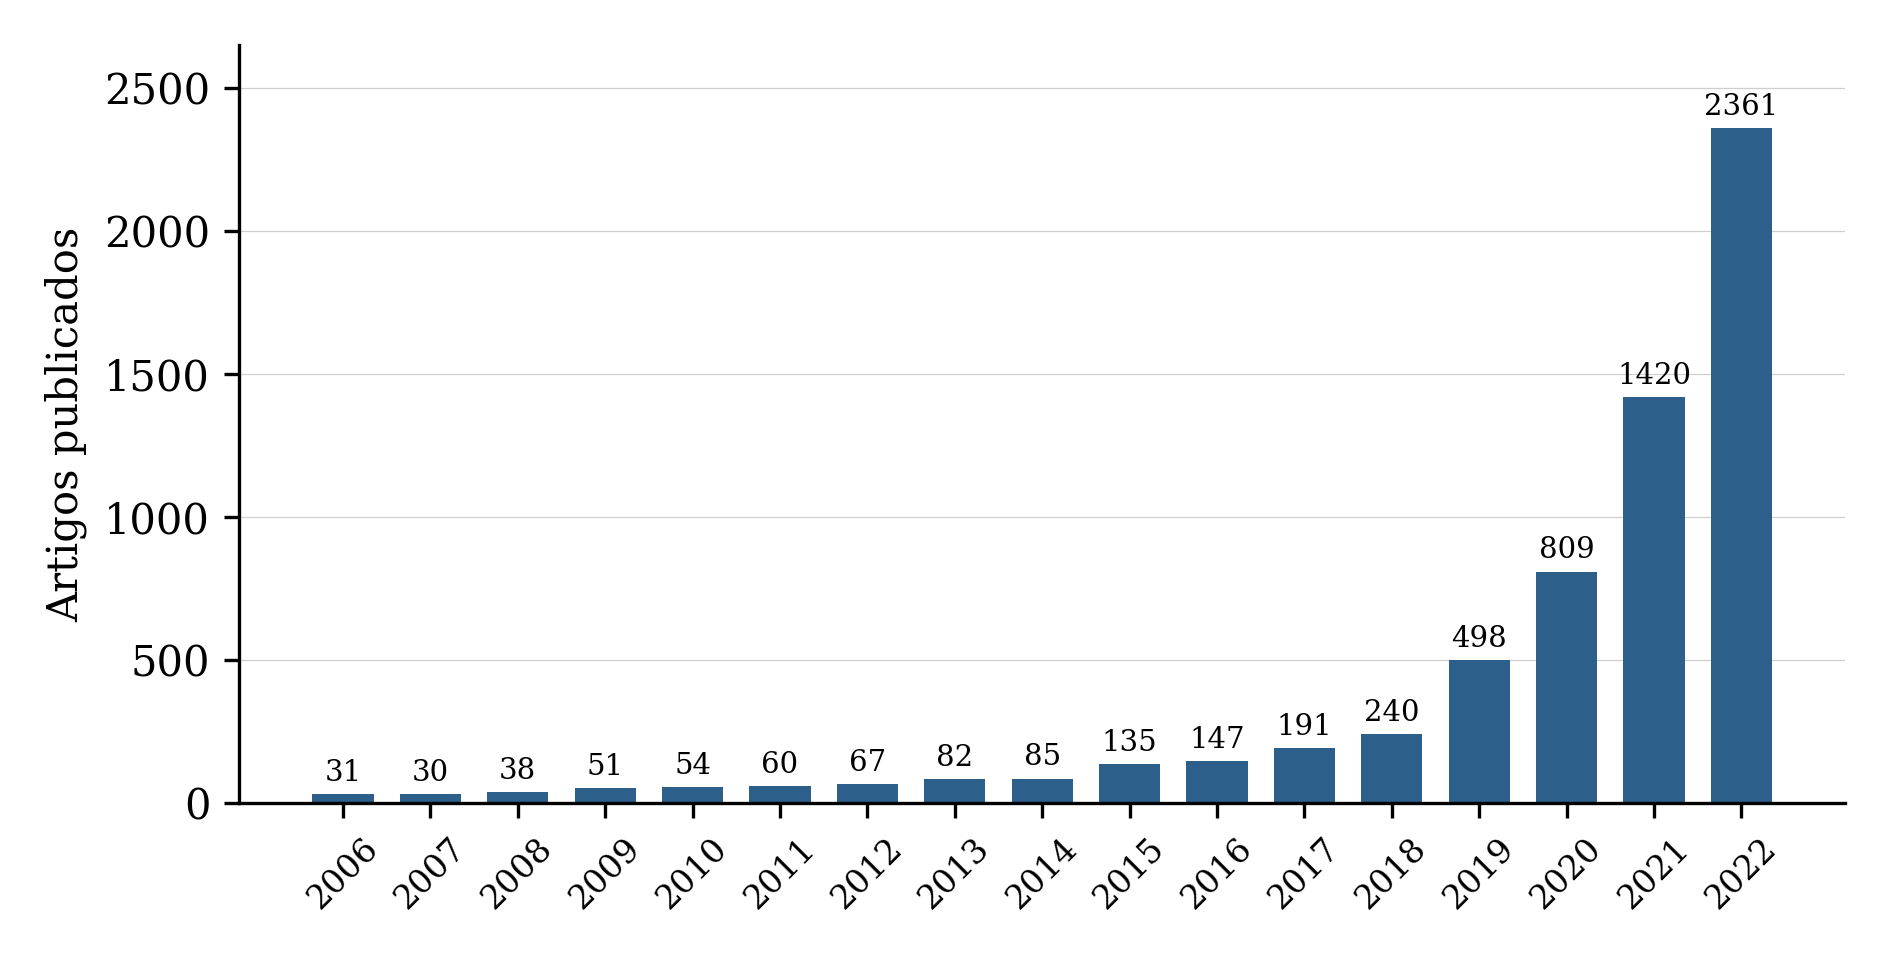
\includegraphics[width=0.85\textwidth]{images/publicacoes_ia_metli.png}
\label{fig:publicacoes_ia}
\legend{Fonte: Elaborado pelo autor com dados de \citeonline{Metli2023}.}
\end{figure}

Dentro desse volume crescente de publicações, foram selecionados sete trabalhos que tratam do uso de IA no ensino e na gestão educacional, descritos a seguir. O primeiro é a revisão sistemática de \citeonline{Tan2025}, que analisou 95 publicações de 2015 a 2024 sobre IA no ensino e no desenvolvimento profissional docente e identificou aplicações em planejamento de aulas, avaliação automatizada, \textit{feedback} individualizado e otimização de tarefas administrativas. Os autores apontam, porém, a escassez de estudos sobre processos administrativos de instituições de ensino superior, lacuna na qual este trabalho se insere.

O trabalho de \citeonline{Kasneci2023}, um ensaio crítico, discute as oportunidades e os desafios dos LLMs na educação. Entre os riscos, os autores destacam a confiança excessiva nas respostas do modelo e a necessidade de supervisão humana e de transparência, preocupações que orientaram a decisão de manter o avaliador humano como responsável pela decisão final no sistema aqui desenvolvido.

Com foco na gestão, \citeonline{Sposato2025} propõe uma taxonomia das aplicações de IA na liderança e na administração de instituições de ensino. A automação de análises documentais aparece nessa taxonomia entre os usos administrativos, mas de forma conceitual, sem a implementação de um sistema.

Já \citeonline{Hoare2025} relatam a experiência do Departamento de Educação de Nova Gales do Sul, na Austrália, que desenvolveu uma ferramenta própria de IA generativa, o NSWEduChat, testada em 50 escolas a partir de 2024 para apoiar práticas de ensino baseadas em evidências. Entre os mais de 100 professores participantes da formação associada, 95\% afirmaram que a ferramenta economizaria tempo. O estudo destaca que a contextualização das respostas com materiais e diretrizes institucionais foi decisiva para a confiança dos docentes, o que apoia a estratégia de fundamentar a avaliação nas normas do IFC.

No contexto brasileiro, \citeonline{Santos2025} analisam a adoção de plataformas digitais e de IA na gestão de redes públicas de ensino e alertam que a centralização dessas plataformas pode restringir a autonomia dos atores escolares, concluindo que uma adoção responsável exige transparência no uso dos dados e infraestrutura adequada.

Mais próximo do contexto deste trabalho, \citeonline{Vieira2025} realizaram uma revisão integrativa sobre IA nos Institutos Federais. Os autores constataram pouca produção acadêmica sobre o tema e identificaram a IA como apoio administrativo como a forma de incorporação menos explorada na rede federal.

Por fim, \citeonline{VieiraFilho2024} aplica técnicas de PLN em Python à recomendação de conteúdo educacional em português. Embora não trate de processos administrativos, o trabalho demonstra a viabilidade dessas técnicas sobre textos acadêmicos no idioma, condição necessária para a abordagem adotada aqui.

A Tabela \ref{tab:relacionados} sintetiza a comparação entre os sete trabalhos descritos nesta seção e a proposta deste trabalho. A análise bibliométrica de \citeonline{Metli2023} não foi incluída na comparação por tratar do volume de publicações sobre o tema, e não de uma aplicação específica de IA.

\begin{table}[H]
\centering
\caption{Comparação entre os trabalhos relacionados e este trabalho}
\label{tab:relacionados}
\footnotesize
\begin{tabular}{@{}L{3.1cm}L{3.4cm}L{2.6cm}L{2.2cm}L{2.4cm}@{}}
\toprule
\rowcolor[HTML]{EFEFEF}
\textbf{Trabalho} & \textbf{Foco} & \textbf{Tipo de estudo} & \textbf{Contexto} & \textbf{Processo administrativo?} \\ \midrule
\citeonline{Tan2025} & IA no ensino e na formação docente & Revisão sistemática & Internacional & Apontado como lacuna \\
\citeonline{Kasneci2023} & Oportunidades e riscos de LLMs na educação & Ensaio crítico & Internacional & Não \\
\citeonline{Sposato2025} & IA na gestão educacional & Taxonomia & Internacional & Sim, conceitual \\
\citeonline{Hoare2025} & Ferramenta institucional de IA generativa & Relato de implantação & Austrália, educação básica & Não \\
\citeonline{Santos2025} & Plataformas e IA na gestão pública & Análise documental & Brasil, redes públicas & Sim, conceitual \\
\citeonline{Vieira2025} & IA nos Institutos Federais & Revisão integrativa & Brasil, rede federal & Apontado como lacuna \\
\citeonline{VieiraFilho2024} & PLN para recomendação de conteúdo & Desenvolvimento de sistema & Brasil, ensino superior & Não \\
\textbf{Este trabalho} & \textbf{Validação de planos de ensino} & \textbf{Sistema e estudo de caso} & \textbf{IFC Videira} & \textbf{Sim, implementado e avaliado} \\ \bottomrule
\end{tabular}
\legend{Fonte: Elaborado pelo autor (2026).}
\end{table}

Os trabalhos revisados confirmam o interesse crescente pela IA na educação, mas tratam a gestão administrativa de forma conceitual ou a apontam como lacuna. Nenhum deles implementa e avalia um sistema para a verificação de planos de ensino frente a normas institucionais. Este trabalho busca contribuir para preencher essa lacuna com uma solução implementada, de baixo custo, executada localmente e avaliada sobre documentos reais de um Instituto Federal da região Sul.


% METODOLOGIA DA PESQUISA
\chapter{METODOLOGIA}
\label{cap:metodologia}

Este capítulo descreve como a pesquisa foi conduzida: sua classificação, as etapas realizadas, o corpus de documentos, os critérios de avaliação, o ambiente experimental, o protocolo de avaliação e os cuidados éticos adotados. O processo de desenvolvimento de software propriamente dito é detalhado na Seção \ref{sec:processo}.

\section{Classificação da pesquisa}

Quanto à natureza, trata-se de uma pesquisa aplicada, pois busca gerar conhecimento para a solução de um problema concreto \cite{Gil2017}: a conferência dos planos de ensino de um curso de graduação. Quanto aos objetivos, é exploratória, por investigar a viabilidade de uma tecnologia ainda pouco aplicada a esse problema, e descritiva, por caracterizar o comportamento do sistema sobre documentos reais \cite{Gil2017}. A abordagem é predominantemente quantitativa, com métricas de desempenho e de concordância, complementada por uma análise qualitativa dos erros.

Quanto ao procedimento, adota-se o estudo de caso, que investiga um fenômeno contemporâneo em seu contexto real \cite{Yin2015}. O caso estudado é a validação dos planos de ensino do curso de Ciência da Computação do IFC -- Campus Videira, e a unidade de análise é o par (plano de ensino, critério de avaliação).

\section{Etapas da pesquisa}

A partir dessa classificação, a pesquisa foi organizada em cinco etapas, relacionadas aos objetivos específicos:

\begin{enumerate}
    \item Levantamento de critérios (primeiro objetivo específico): leitura da Organização Didática do IFC \cite{ifc2022} e dos planos exportados pelo SIGAA, e definição, em conjunto com o orientador, dos critérios de avaliação e de suas regras.
    \item Projeto e implementação (segundo e terceiro objetivos específicos): desenvolvimento iterativo do fluxo de validação e do painel \textit{web}, descrito no Capítulo \ref{cap:desenvolvimento}.
    \item Execuções sobre o corpus: processamento repetido dos planos de ensino a cada nova versão do sistema, com registro de todos os resultados.
    \item Avaliação (quarto objetivo específico): cálculo das métricas de robustez, desempenho e concordância e análise dos erros.
    \item Redação: consolidação dos resultados e elaboração deste documento.
\end{enumerate}

\section{Corpus}
\label{sec:corpus}

As etapas de execução e de avaliação foram realizadas sobre um mesmo conjunto de documentos. O corpus é formado pelos 29 planos de ensino do semestre letivo 2024/1 do curso de Ciência da Computação disponibilizados em uma pasta do Google Drive para este trabalho. Todos foram exportados do SIGAA em PDF com texto pesquisável, o que dispensou o reconhecimento óptico de caracteres. Os documentos têm entre 3 e 5 páginas (média de 3,4) e, após a extração, entre 4.520 e 11.436 caracteres (média de 7.048, desvio-padrão de 1.700). Entre os componentes curriculares há disciplinas de formação básica, como matemática e estatística, de formação tecnológica, como programação, banco de dados e redes, e de formação complementar, como metodologia científica e trabalho de conclusão de curso. Dois planos correspondem a turmas distintas de um mesmo componente, o que permitiu observar a consistência do sistema diante de documentos quase idênticos.

A avaliação detalhada descrita na Seção \ref{sec:protocolo} usa esse corpus de 2024/1. Ao final do trabalho, o orientador disponibilizou também os planos de 2024/2, 2025/1 e 2025/2, e o sistema foi executado sobre os quatro semestres, totalizando 120 planos processados. Essa ampliação, apresentada na Seção \ref{sec:res-semestres}, mede a estabilidade do sistema e a evolução da conformidade dos planos, mas não repete a conferência manual de todos os apontamentos.

\section{Critérios de avaliação}
\label{sec:criterios}

Sobre cada plano do corpus, o sistema verifica um conjunto de critérios. Esses critérios foram definidos a partir dos elementos exigidos pela Organização Didática \cite{ifc2022} e das orientações do orientador deste trabalho, que sugeriu a lista inicial de itens a verificar e participou dos ajustes posteriores. Dois ajustes merecem registro. O item ``adequação à ementa'' foi incorporado ao critério de coerência, por se sobrepor a ele. A exigência de que os procedimentos de avaliação mencionassem a interdisciplinaridade foi removida, pois as primeiras execuções mostraram que ela levava o modelo a reprovar planos que descreviam adequadamente seus instrumentos de avaliação. Os doze critérios resultantes e suas regras estão na Tabela \ref{tab:criterios}.

\begin{table}[H]
\centering
\caption{Critérios de avaliação e regras de conformidade}
\label{tab:criterios}
\footnotesize
\begin{tabular}{@{}L{3.3cm}L{9.0cm}L{2.0cm}@{}}
\toprule
\rowcolor[HTML]{EFEFEF}
\textbf{Critério} & \textbf{Regra para o status OK} & \textbf{Avaliado por} \\ \midrule
Identificação & Contém o nome da instituição, do componente curricular e do docente & LLM \\
Ementa & Descreve os temas da disciplina em texto corrido com ao menos 15 palavras & LLM \\
Objetivo geral & Possui texto preenchido & Regra \\
Objetivos específicos & Possuem texto preenchido & Regra \\
Conteúdo programático & Lista os tópicos ou unidades de conteúdo & LLM \\
Metodologia & Descreve como as aulas serão conduzidas (estratégias e recursos) & LLM \\
Procedimentos de avaliação & Descreve os instrumentos de avaliação & LLM \\
Cronograma & Apresenta distribuição temporal dos conteúdos (datas ou semanas) & LLM \\
Avaliações & Indica as avaliações previstas (instrumentos, datas ou pesos) & LLM \\
Horário de atendimento & Informa dia(s) e/ou horário(s) de atendimento ao estudante & LLM \\
Referências & No mínimo 3 referências básicas e 5 complementares & Regra \\
Coerência & Objetivos, metodologia e avaliação compatíveis entre si & LLM \\ \bottomrule
\end{tabular}
\legend{Fonte: Elaborado pelo autor (2026), com base em \citeonline{ifc2022}.}
\end{table}

Cada critério recebe um entre três status: OK, quando atende à regra; INCOMPLETO, quando há conteúdo relacionado que não atende à regra; e AUSENTE, quando o campo está vazio ou sem relação com o critério. O plano recebe um status geral: OK, se todos os critérios estão OK; PENDENTE, se há ao menos um critério INCOMPLETO e nenhum AUSENTE; e REPROVADO, se há ao menos um critério AUSENTE. Falhas técnicas que impeçam a avaliação geram o status ERRO.

\section{Ambiente experimental}

Para que os resultados de desempenho possam ser interpretados e reproduzidos, é preciso registrar o equipamento em que foram obtidos. Todas as execuções foram realizadas em um computador portátil, com os componentes descritos na Tabela \ref{tab:ambiente}. O modelo de linguagem foi executado inteiramente no equipamento local, sem envio dos documentos a serviços de IA externos.

\begin{table}[H]
\centering
\caption{Ambiente experimental}
\label{tab:ambiente}
\footnotesize
\begin{tabular}{@{}L{4.2cm}L{10.2cm}@{}}
\toprule
\rowcolor[HTML]{EFEFEF}
\textbf{Componente} & \textbf{Especificação} \\ \midrule
Processador & Intel Core Ultra 7 155H \\
Memória RAM & 32 GB \\
GPU & NVIDIA GeForce RTX 4050 Laptop, 6 GB de VRAM \\
Sistema operacional & Windows 11, com Docker Desktop \\
Orquestração & n8n 2.21.7 (contêiner \texttt{docker.n8n.io/n8nio/n8n}) \\
Servidor de inferência & Ollama 0.24.0 (contêiner \texttt{ollama/ollama}) \\
Modelo de linguagem & Qwen2.5 7B Instruct, 7,6 bilhões de parâmetros, quantização Q4\_K\_M \\
Parâmetros de geração & temperatura 0,1; contexto de 8.192 \textit{tokens}; máximo de 1.500 \textit{tokens} gerados \\
Otimizações do Ollama & \textit{FlashAttention} ativado; \textit{KV cache} quantizado em 8 bits (\texttt{q8\_0}) \\
Armazenamento & Google Drive (planos) e Google Sheets (resultados) nas execuções avaliadas; pastas locais na versão final (Seção \ref{sec:apresentacao}) \\ \bottomrule
\end{tabular}
\legend{Fonte: Elaborado pelo autor (2026).}
\end{table}

A temperatura de 0,1 foi escolhida para tornar as respostas praticamente determinísticas, característica desejável em uma tarefa de verificação, na qual o mesmo documento deve receber a mesma avaliação em execuções diferentes.

\section{Protocolo de avaliação}
\label{sec:protocolo}

Definidos o corpus, os critérios e o ambiente, resta descrever como o sistema foi avaliado, o que corresponde ao quarto objetivo específico. A avaliação foi organizada em quatro dimensões, cada uma com uma fonte de dados e uma medida próprias, descritas a seguir.

Robustez técnica. Neste trabalho, robustez técnica é a capacidade do sistema de processar todos os planos do lote sem falhas que impeçam a avaliação, como respostas vazias, JSON inválido ou estouro do tempo limite. Ela foi medida pela proporção de planos que receberam o status ERRO em cada execução sobre o corpus, acompanhada do motivo da falha registrado pelo sistema. Como a planilha de resultados usada durante o desenvolvimento acumulou todas as execuções, foi possível reconstruir a evolução dessa proporção ao longo das iterações de desenvolvimento e associar cada queda a uma correção específica.

Desempenho computacional. Para cada requisição ao modelo, o Ollama informa o número de \textit{tokens} de entrada e de saída e o tempo gasto em cada fase. Esses metadados, preservados no histórico de execuções do n8n, foram usados para calcular o tempo de inferência por plano, a velocidade de geração em \textit{tokens} por segundo e o tempo total de processamento do lote.

Concordância com oráculo estrutural. Para o critério de horário de atendimento, a presença de conteúdo pode ser verificada de forma objetiva no texto extraído: no modelo do SIGAA, o rótulo ``Horário de Atendimento'' é seguido imediatamente pela seção ``Programa'', e o texto entre os dois indica se o campo foi preenchido. Esse oráculo estrutural, implementado no \textit{script} do Apêndice \ref{ap:analise}, serve como referência independente do modelo de linguagem para o cálculo das métricas da Seção \ref{sec:metricas}. Para os critérios de referências e de objetivos, avaliados por regras determinísticas, verificou-se por amostragem, no texto extraído, se as contagens e detecções correspondiam ao conteúdo dos documentos.

Análise de erros. Todos os planos com algum critério diferente de OK na execução final foram confrontados com o texto extraído do PDF, classificando cada apontamento como correto ou incorreto e identificando a causa dos erros.

Para os critérios que dependem de interpretação, como metodologia e coerência, não existe oráculo estrutural, e a referência adequada é o parecer de avaliadores humanos. O protocolo previsto para essa comparação consiste em: (i) solicitar a membros do NDE que classifiquem, de forma independente e sem acesso à saída do sistema, cada critério de cada plano; (ii) consolidar os pareceres em uma referência única, resolvendo divergências por consenso; e (iii) calcular, por critério, precisão, \textit{recall}, $F_1$ e Kappa de Cohen entre o sistema e a referência. Os artefatos necessários para executar esse protocolo, a planilha de anotação e o \textit{script} de cálculo das métricas, foram produzidos e estão descritos no Apêndice \ref{ap:analise}. A realização da anotação pelo NDE não coube no período deste trabalho e é discutida como limitação no Capítulo \ref{cap:conclusao}.

\section{Aspectos éticos}

Por trabalhar com documentos reais, a pesquisa exigiu cuidados com a exposição das pessoas envolvidas. Os planos de ensino são documentos institucionais de caráter público para a comunidade acadêmica, mas contêm o nome dos docentes responsáveis. Para evitar qualquer exposição individual, os resultados deste trabalho são apresentados de forma anonimizada: os planos são identificados por códigos de P01 a P29, atribuídos pela ordem alfabética do nome do arquivo, e nenhuma tabela associa resultados a docentes ou a componentes curriculares. O processamento foi realizado em equipamento local, sem envio dos documentos a provedores externos de IA, em consonância com os princípios de finalidade e de necessidade da LGPD \cite{Brasil2018}. Os resultados do sistema têm caráter indicativo e não foram utilizados para qualquer decisão sobre os planos avaliados.


% DESENVOLVIMENTO DO SISTEMA
\chapter{DESENVOLVIMENTO}
\label{cap:desenvolvimento}

Este capítulo documenta o sistema desenvolvido. A Seção \ref{sec:apresentacao} apresenta uma visão geral da solução e a Seção \ref{sec:processo} descreve o processo de desenvolvimento adotado. As Seções \ref{sec:rf} a \ref{sec:historias} especificam os requisitos, os atores, as regras de negócio e as histórias de usuário. A Seção \ref{sec:bd} apresenta a modelagem de dados, a Seção \ref{sec:diagramas} reúne os diagramas estruturais e comportamentais, a Seção \ref{sec:implementacao} detalha a implementação de cada etapa e a Seção \ref{sec:prototipo} apresenta a interface. Por fim, a Seção \ref{sec:testes} descreve a estratégia de testes.

\section{Apresentação do Sistema}
\label{sec:apresentacao}

O sistema desenvolvido é um conjunto de dois fluxos de automação executados na plataforma n8n, apoiados por um servidor de modelos de linguagem local. O fluxo de validação lê os planos de ensino em PDF de uma pasta local, extrai e segmenta o texto de cada plano, solicita ao modelo de linguagem a avaliação dos critérios, aplica regras determinísticas sobre a resposta e grava o resultado de cada plano em um arquivo JSON, em outra pasta local. O fluxo do \textit{dashboard} lê esses arquivos e gera, a cada acesso, uma página HTML com os indicadores do lote, o detalhamento de cada plano e a exportação dos resultados em CSV.

A Figura \ref{fig:arquitetura} apresenta a arquitetura da solução. Os dois serviços próprios, n8n e Ollama, são executados em contêineres Docker orquestrados por um arquivo Docker Compose e se comunicam por uma rede interna. O Ollama tem acesso à GPU do computador hospedeiro, onde o modelo Qwen2.5 é carregado. Duas pastas do computador hospedeiro são montadas no contêiner do n8n: a pasta \texttt{planos}, repositório de entrada onde a coordenação deposita os PDFs, e a pasta \texttt{resultados}, onde o sistema grava as validações. Dessa forma, o sistema não depende de serviços externos nem de credenciais, e a implantação se resume a iniciar os contêineres, importar os fluxos e copiar os planos para a pasta de entrada. Até a penúltima iteração, a entrada e a saída usavam o Google Drive e o Google Sheets, acessados por OAuth 2.0. Essa configuração exigia, a cada implantação, criar um projeto no Google Cloud, ativar as APIs, configurar a tela de consentimento e cadastrar as credenciais no n8n, etapa apontada na revisão do orientador como complexa demais para a adoção do sistema, e por isso foi substituída pelo armazenamento local.

\begin{figure}[htbp]
\centering
\caption{Arquitetura do sistema}
\label{fig:arquitetura}
\begin{tikzpicture}[every node/.style={font=\footnotesize}]
  % Linha 1: entrada, validação e modelo
  \node[ext, text width=2.4cm] (drive) at (0,2) {Pasta \texttt{planos}\\\scriptsize PDFs dos planos};
  \node[caixa, text width=3.9cm] (wfval) at (5.4,2) {\textbf{Workflow de validação}\\\scriptsize busca, extração, segmentação, \textit{prompt}, interpretação e registro};
  \node[ia, text width=2.7cm] (llm) at (11.0,2) {\textbf{Ollama}\\\scriptsize Qwen2.5 7B (Q4\_K\_M)\\\texttt{/api/generate}};
  \node[caixa, text width=2.7cm, font=\scriptsize] (gpu) at (11.0,0.25) {GPU NVIDIA (6 GB)};

  % Linha 2: resultados e dashboard
  \node[ext, text width=2.4cm] (sheets) at (0,-1.4) {Pasta \texttt{resultados}\\\scriptsize um JSON por plano};
  \node[caixa, text width=3.9cm] (wfdash) at (5.4,-1.4) {\textbf{Workflow do \textit{dashboard}}\\\scriptsize leitura dos resultados, HTML e CSV};

  % Linha 3: usuário
  \node[caixa, text width=3.9cm] (user) at (5.4,-4.2) {Coordenação, NDE ou docente\\\scriptsize navegador \textit{web}};

  % Agrupamentos
  \begin{scope}[on background layer]
    \node[grupo, fit=(wfval)(wfdash), inner sep=10pt] (n8n) {};
    \node[grupo, fit=(llm)(gpu), inner sep=10pt] (oll) {};
    \node[draw, rounded corners=4pt, black!80, fit=(n8n)(oll), inner sep=8pt] (docker) {};
  \end{scope}
  \node[font=\scriptsize\bfseries, anchor=south] at (n8n.north) {Contêiner n8n};
  \node[font=\scriptsize\bfseries, anchor=south] at (oll.north) {Contêiner Ollama};
  \node[font=\scriptsize\bfseries, anchor=south west] at ([yshift=1mm]docker.north west) {Docker Compose -- rede interna \texttt{tc-network}};

  % Fluxos
  \draw[seta] (drive) -- node[rotulo, above]{1. lê PDFs} (wfval);
  \draw[seta] ([yshift=2.5mm]wfval.east) -- node[rotulo, above]{2. \textit{prompt} + esquema} ([yshift=2.5mm]llm.west);
  \draw[seta] ([yshift=-2.5mm]llm.west) -- node[rotulo, below]{3. JSON} ([yshift=-2.5mm]wfval.east);
  \draw[thick, dotted] (llm) -- (gpu);
  \draw[seta] (wfval.south west) -- node[rotulo, above, sloped]{4. um arquivo por plano} (sheets.north east);
  \draw[seta] (sheets) -- node[rotulo, above]{5. leitura} (wfdash);
  \draw[seta, {Stealth[length=2.2mm]}-{Stealth[length=2.2mm]}] (user) -- node[rotulo, right]{6. \texttt{GET /webhook/dashboard}} (wfdash);
\end{tikzpicture}

\legend{Fonte: Elaborado pelo autor (2026).}
\end{figure}

Três princípios orientaram o projeto. O primeiro é a divisão de trabalho entre regras e modelo: o que pode ser verificado de forma exata, como contar referências, é feito por código, e o LLM é reservado aos julgamentos que exigem interpretação. O segundo é a verificabilidade: cada critério recebe um status de um conjunto fechado e uma observação curta, e o \textit{dashboard} oferece acesso direto ao PDF original. O terceiro é o controle humano: o sistema faz uma triagem e não toma decisões, cabendo à coordenação e ao NDE confirmar ou descartar cada apontamento.

\section{Metodologia de desenvolvimento de software}
\label{sec:processo}

A solução apresentada na seção anterior não foi definida de uma só vez, mas construída ao longo de várias versões. O desenvolvimento seguiu um processo iterativo e incremental, no qual o sistema é construído em versões sucessivas e cada versão é avaliada antes de orientar a seguinte \cite{Sommerville2016, Pressman2016}. A escolha se justifica pelo caráter exploratório do projeto: não era possível prever, antes de executar o sistema sobre planos reais, como o modelo de linguagem se comportaria diante dos documentos, quais regras seriam ambíguas ou quais limites de infraestrutura seriam atingidos. Em linha com os valores do Manifesto Ágil \cite{Beck2001}, privilegiou-se ter software funcionando desde a primeira iteração e responder às mudanças identificadas nas execuções, em vez de seguir um plano fechado.

Cada iteração seguiu o mesmo ciclo: (i) executar a versão corrente sobre o corpus completo; (ii) inspecionar, nos resultados gravados e no histórico de execuções do n8n, os resultados e as falhas; (iii) identificar a causa raiz do problema mais grave; e (iv) implementar e documentar a correção. O código dos fluxos, exportado do n8n em formato JSON, e a configuração da infraestrutura foram versionados com Git em um repositório no GitHub, e um arquivo de documentação registrou as instruções de instalação e os problemas conhecidos com suas soluções. A Tabela \ref{tab:iteracoes} resume as iterações realizadas.

\begin{table}[H]
\centering
\caption{Iterações de desenvolvimento}
\label{tab:iteracoes}
\footnotesize
\begin{tabular}{@{}L{2.4cm}L{9.1cm}L{2.9cm}@{}}
\toprule
\rowcolor[HTML]{EFEFEF}
\textbf{Período} & \textbf{Principais entregas e correções} & \textbf{Execução de referência} \\ \midrule
Maio/2026 & Primeira versão do fluxo: busca no Drive, extração de texto, avaliação do plano pelo LLM e registro na planilha & 22/05: 86,2\% de ERRO \\
Julho/2026 & Critérios definidos com o orientador; segmentação do texto por seções; \textit{dashboard} HTML; suporte a GPU; documentação de instalação & 07/07: 3,4\% de ERRO \\
Agosto/2026 & Processamento em blocos com uma requisição por vez e retentativas; adoção do Qwen2.5 7B; correção do contexto máximo do modelo (de 4.096 para 12.288 \textit{tokens}) & 10/08: 69,0\%; 25/08: 49,1\% de ERRO \\
Setembro/2026 & Contagem determinística de referências; regras determinísticas para objetivos e status geral; remoção da exigência de interdisciplinaridade & 10/09: 0\%; 15/09: 17,2\% de ERRO \\
Outubro/2026 & Segmentação ancorada no início da linha; contexto de 8.192 \textit{tokens}; \textit{FlashAttention} e \textit{KV cache} em 8 bits; \textit{timeout} de 180 s & 19/10: 0\% de ERRO \\
Novembro/2026 & Armazenamento local: planos lidos de uma pasta e resultados gravados em arquivos JSON, em substituição ao Google Drive e ao Google Sheets; exportação em CSV e abertura do PDF pelo \textit{dashboard} & Teste funcional do fluxo, sem nova execução sobre o corpus \\ \bottomrule
\end{tabular}
\legend{Fonte: Elaborado pelo autor (2026), com base no histórico de execuções e na planilha de resultados.}
\end{table}

Os problemas encontrados em cada iteração e o efeito das correções são analisados na Seção \ref{sec:res-robustez}.

\section{Requisitos Funcionais}
\label{sec:rf}

Os requisitos funcionais descrevem os serviços que o sistema deve oferecer \cite{Sommerville2016}. Eles foram levantados a partir do processo manual de conferência e refinados ao longo das iterações. A Tabela \ref{tab:rf} apresenta os requisitos funcionais implementados.

\begin{table}[H]
\centering
\caption{Requisitos funcionais}
\label{tab:rf}
\footnotesize
\begin{tabular}{@{}L{1.1cm}L{13.3cm}@{}}
\toprule
\rowcolor[HTML]{EFEFEF}
\textbf{Nº} & \textbf{Descrição do Requisito Funcional} \\ \midrule
RF01 & O sistema deve ler os arquivos PDF de uma pasta local configurada, ignorando arquivos de outros tipos. \\
RF02 & O sistema deve extrair o texto de cada plano de ensino em PDF. \\
RF03 & O sistema deve segmentar o texto nas seções do plano: identificação, ementa, metodologia, procedimentos de avaliação, horário de atendimento, objetivo geral, objetivos específicos, conteúdo programático, cronograma, avaliações e referências. \\
RF04 & O sistema deve contar as referências básicas e complementares de cada plano. \\
RF05 & O sistema deve avaliar os doze critérios da Tabela \ref{tab:criterios}, atribuindo a cada um o status OK, INCOMPLETO ou AUSENTE e uma observação. \\
RF06 & O sistema deve calcular o status geral do plano (OK, PENDENTE ou REPROVADO) a partir dos status dos critérios. \\
RF07 & O sistema deve registrar o status ERRO e o motivo da falha quando não for possível avaliar um plano. \\
RF08 & O sistema deve gravar o resultado de cada plano em um arquivo na pasta de resultados, com data e hora da validação e o \textit{link} para o PDF original. \\
RF09 & O sistema deve executar a validação automaticamente uma vez por dia e permitir a execução manual. \\
RF10 & O sistema deve disponibilizar um \textit{dashboard} com o total de planos e as quantidades e percentuais de planos aprovados, pendentes e com problemas. \\
RF11 & O \textit{dashboard} deve exibir, para cada plano, o status e a observação de cada critério. \\
RF12 & O \textit{dashboard} deve permitir abrir o PDF original de cada plano. \\
RF13 & O sistema deve permitir trocar o modelo de linguagem utilizado, inclusive por um serviço externo. \\
RF14 & O \textit{dashboard} deve permitir exportar todos os resultados em formato CSV. \\ \bottomrule
\end{tabular}
\legend{Fonte: Elaborado pelo autor (2026).}
\end{table}

\section{Requisitos Não Funcionais}
\label{sec:rnf}

Enquanto os requisitos funcionais definem o que o sistema faz, os requisitos não funcionais expressam restrições e qualidades do sistema \cite{Sommerville2016}. Eles foram organizados segundo as características de qualidade da norma ISO/IEC 25010 \cite{ISO25010} e estão na Tabela \ref{tab:rnf}.

\begin{table}[H]
\centering
\caption{Requisitos não funcionais}
\label{tab:rnf}
\footnotesize
\begin{tabular}{@{}L{1.2cm}L{2.8cm}L{10.4cm}@{}}
\toprule
\rowcolor[HTML]{EFEFEF}
\textbf{Nº} & \textbf{Característica} & \textbf{Descrição do Requisito Não Funcional} \\ \midrule
RNF01 & Segurança & O conteúdo dos planos não deve ser enviado a serviços externos de IA na configuração padrão; o modelo deve ser executado localmente. \\
RNF02 & Segurança & Os fluxos devem ter acesso apenas às pastas de planos e de resultados, e a configuração padrão não deve depender de credenciais de serviços externos. \\
RNF03 & Eficiência de desempenho & O sistema deve validar um lote de 30 planos em menos de 30 minutos no ambiente da Tabela \ref{tab:ambiente}. \\
RNF04 & Eficiência de desempenho & O sistema deve operar com uma GPU de 6 GB de VRAM. \\
RNF05 & Confiabilidade & A falha na avaliação de um plano não deve interromper o processamento dos demais. \\
RNF06 & Confiabilidade & Requisições ao modelo devem ser repetidas até 3 vezes em caso de falha, com limite de tempo por requisição. \\
RNF07 & Confiabilidade & Os resultados de cada bloco de planos devem ser gravados antes do processamento do bloco seguinte. \\
RNF08 & Adequação funcional & A resposta do modelo deve seguir um esquema JSON com campos e valores predefinidos. \\
RNF09 & Usabilidade & O \textit{dashboard} deve funcionar em navegadores atuais, sem instalação, e indicar o status por cor e por texto. \\
RNF10 & Portabilidade & O sistema deve ser implantável com Docker Compose em Windows, Linux ou macOS; a GPU deve ser opcional. \\
RNF11 & Manutenibilidade & As regras de avaliação e o modelo devem ser configuráveis em um único ponto do fluxo. \\
RNF12 & Manutenibilidade & Os fluxos e a infraestrutura devem ser versionados em repositório Git. \\ \bottomrule
\end{tabular}
\legend{Fonte: Elaborado pelo autor (2026).}
\end{table}

\section{Atores do Sistema}
\label{sec:atores}

Os requisitos descritos nas seções anteriores atendem a diferentes perfis de usuário. A Tabela \ref{tab:atores} apresenta esses usuários e o que cada um pode fazer no sistema. Além deles, o agendador do n8n atua como ator temporal, disparando a validação diariamente.

\begin{table}[H]
\centering
\caption{Atores do sistema}
\label{tab:atores}
\footnotesize
\begin{tabular}{@{}L{1.1cm}L{3.4cm}L{9.9cm}@{}}
\toprule
\rowcolor[HTML]{EFEFEF}
\textbf{Nº} & \textbf{Nome} & \textbf{Descrição} \\ \midrule
US1 & Coordenação de curso / NDE & Deposita os planos na pasta de entrada, dispara ou aguarda a validação, consulta o \textit{dashboard}, analisa os apontamentos e decide sobre cada plano. \\
US2 & Docente & Consulta o resultado do próprio plano no \textit{dashboard}, identifica os itens apontados e reenvia o plano corrigido. \\
US3 & Administrador técnico & Instala e mantém a infraestrutura, configura as pastas de planos e de resultados e o modelo de linguagem, e acompanha as execuções no n8n. \\ \bottomrule
\end{tabular}
\legend{Fonte: Elaborado pelo autor (2026).}
\end{table}

\section{Regras de Negócio}
\label{sec:rn}

Além do que cada ator pode fazer, é preciso definir como o sistema deve decidir. As regras de negócio orientam e controlam esse comportamento. Elas derivam da Organização Didática \cite{ifc2022}, das orientações da coordenação e das decisões tomadas durante as iterações:

\begin{itemize}
    \item RN01 -- Cada critério recebe exatamente um status entre OK, INCOMPLETO e AUSENTE; havendo conteúdo relacionado ao critério, o status AUSENTE não deve ser usado.
    \item RN02 -- O plano é REPROVADO se algum critério estiver AUSENTE; PENDENTE se algum estiver INCOMPLETO e nenhum AUSENTE; e OK se todos estiverem OK.
    \item RN03 -- O critério de referências é conforme somente com no mínimo 3 referências básicas e 5 complementares, contadas pelo sistema e não pelo modelo.
    \item RN04 -- Os critérios de objetivo geral e de objetivos específicos são conformes quando possuem texto preenchido, independentemente da redação.
    \item RN05 -- Os procedimentos de avaliação não são considerados incompletos pela ausência de menção à interdisciplinaridade.
    \item RN06 -- A avaliação de cada critério deve se basear apenas no texto do plano, sem inferência de informações ausentes.
    \item RN07 -- O status calculado pelo sistema é indicativo; a decisão sobre o plano cabe à coordenação e ao NDE.
    \item RN08 -- Uma falha técnica na avaliação de um plano gera o status ERRO, com o motivo registrado, e o plano deve ser reavaliado em nova execução.
\end{itemize}

\section{Histórias de Usuário}
\label{sec:historias}

Os requisitos, os atores e as regras de negócio foram reunidos, do ponto de vista dos usuários, em histórias de usuário. As histórias de usuário descrevem funcionalidades do ponto de vista de quem as utiliza, no formato ``como \textless papel\textgreater, quero \textless funcionalidade\textgreater, para \textless benefício\textgreater'', acompanhadas de critérios de aceitação \cite{Cohn2004}. A Tabela \ref{tab:historias} relaciona as histórias que representam o escopo implementado.

\begin{table}[H]
\centering
\caption{Histórias de usuário}
\label{tab:historias}
\footnotesize
\begin{tabular}{@{}L{1.1cm}L{7.0cm}L{6.3cm}@{}}
\toprule
\rowcolor[HTML]{EFEFEF}
\textbf{Nº} & \textbf{História} & \textbf{Critérios de aceitação} \\ \midrule
HU01 & Como coordenador, quero validar todos os planos de uma pasta de uma só vez, para não precisar abrir documento por documento. & Todos os PDFs da pasta geram um registro de resultado; arquivos de outros tipos são ignorados. (RF01, RF02, RF08) \\
HU02 & Como coordenador, quero ver quantos planos estão aprovados, pendentes ou com problemas, para dimensionar o trabalho de revisão. & O \textit{dashboard} exibe total, quantidades e percentuais por status. (RF10) \\
HU03 & Como membro do NDE, quero ver o status e a justificativa de cada critério de um plano, para revisar apenas os itens apontados. & Ao expandir um plano, os doze critérios aparecem com status, cor e observação. (RF05, RF11) \\
HU04 & Como membro do NDE, quero abrir o PDF original a partir do resultado, para confirmar ou descartar um apontamento. & Cada plano possui um \textit{link} que abre o arquivo original no navegador. (RF12) \\
HU05 & Como coordenador, quero que a contagem de referências seja exata, para cobrar o mínimo exigido com segurança. & A observação informa a quantidade de referências básicas e complementares encontradas. (RF04, RN03) \\
HU06 & Como coordenador, quero que a validação rode sozinha todos os dias, para que planos novos sejam avaliados sem intervenção. & O fluxo é disparado diariamente às 5h. (RF09) \\
HU07 & Como docente, quero saber exatamente o que falta no meu plano, para corrigi-lo antes do prazo. & Cada critério não conforme tem observação que indica o problema. (RF05, RF11) \\
HU08 & Como administrador, quero que uma falha em um plano não interrompa os demais e fique registrada, para reprocessar apenas o necessário. & O plano com falha recebe status ERRO com o motivo; os demais seguem. (RF07, RNF05) \\
HU09 & Como administrador, quero trocar o modelo de linguagem em um único lugar, para testar modelos maiores ou um serviço externo. & O modelo é definido por uma constante no nó de preparação do \textit{prompt}. (RF13, RNF11) \\
HU10 & Como coordenador, quero levar os resultados para uma planilha eletrônica, para filtrá-los e compartilhá-los. & O \textit{dashboard} oferece o \textit{download} de um arquivo CSV com todos os resultados. (RF14) \\ \bottomrule
\end{tabular}
\legend{Fonte: Elaborado pelo autor (2026).}
\end{table}

\section{Modelagem do Banco de Dados}
\label{sec:bd}

As funcionalidades descritas nas histórias de usuário dependem de dados persistidos, como os resultados de cada validação. O sistema não utiliza um sistema gerenciador de banco de dados relacional: os resultados são armazenados em arquivos JSON na pasta \texttt{resultados}, um arquivo por plano, nomeado a partir do nome do PDF. A escolha elimina a infraestrutura de banco de dados e as credenciais de serviços externos, e a exportação em CSV oferecida pelo \textit{dashboard} permite que a coordenação consulte, filtre e compartilhe os resultados em uma planilha eletrônica já conhecida. Os planos de ensino, por sua vez, permanecem na pasta \texttt{planos}.

A Figura \ref{fig:dados} apresenta o modelo conceitual dos dados. Um plano de ensino pode ser avaliado em várias execuções, e cada validação compõe-se de exatamente doze resultados de critério e de uma contagem de referências.

\begin{figure}[htbp]
\centering
\caption{Modelo conceitual dos dados}
\label{fig:dados}
\begin{tikzpicture}[every node/.style={font=\scriptsize}]
  \tikzset{
    ent/.style={draw, rectangle split, rectangle split parts=2, align=left, fill=white, text width=4.4cm, inner sep=4pt},
  }
  \node[ent] (plano) at (0,0) {\centering\textbf{PlanoDeEnsino}\nodepart{second}
    arquivo: texto (nome no Drive)\\
    link\_pdf: URL\\
    id\_drive: texto};
  \node[ent] (val) at (8.0,0) {\centering\textbf{Validação}\nodepart{second}
    data\_validacao: data e hora\\
    status\_geral: \{OK, PENDENTE,\\\hspace{1.2em}REPROVADO, ERRO\}\\
    observacao\_geral: texto};
  \node[ent] (crit) at (8.0,-3.8) {\centering\textbf{ResultadoCritério}\nodepart{second}
    criterio: \{Identificação, Ementa, \ldots,\\\hspace{1.2em}Coerência\} (12 valores)\\
    status: \{OK, INCOMPLETO,\\\hspace{1.2em}AUSENTE, ERRO\}\\
    observacao: texto};
  \node[ent] (cont) at (0,-3.8) {\centering\textbf{ContagemReferências}\nodepart{second}
    ref\_basicas: inteiro\\
    ref\_complementares: inteiro};

  \draw[thick] (plano.east) -- node[above, pos=0.08]{1} node[above, pos=0.9]{0..*} node[below, midway]{é avaliado em} (val.west);
  \draw[thick] (val.south) -- node[right, pos=0.12]{1} node[right, pos=0.85]{12} node[left, midway]{compõe-se de} (crit.north);
  \draw[thick] (val.south west) -- node[above, pos=0.1]{1} node[above, pos=0.9]{1} node[above, sloped, midway]{deriva} (cont.north east);
\end{tikzpicture}

\legend{Fonte: Elaborado pelo autor (2026).}
\end{figure}

Na implementação, esse modelo é desnormalizado em um único registro por plano, em que os doze resultados de critério são representados por pares de campos (status e observação), totalizando 29 campos, descritos na Tabela \ref{tab:colunas}. A desnormalização simplifica a gravação, feita com a escrita de um único arquivo por plano, e a leitura pelo \textit{dashboard}. Como o arquivo de um plano é sobrescrito a cada nova validação, a pasta reflete sempre o resultado mais recente de cada plano, sem registros duplicados. Durante o desenvolvimento, quando os resultados eram gravados no Google Sheets, cada execução acrescentava novas linhas sem apagar as anteriores, e foi esse histórico acumulado que permitiu reconstruir a evolução do sistema apresentada no Capítulo \ref{cap:resultados}.

\begin{table}[H]
\centering
\caption{Estrutura do registro de resultado de cada plano}
\label{tab:colunas}
\footnotesize
\begin{tabular}{@{}L{4.6cm}L{2.0cm}L{7.8cm}@{}}
\toprule
\rowcolor[HTML]{EFEFEF}
\textbf{Campo} & \textbf{Tipo} & \textbf{Conteúdo} \\ \midrule
Arquivo & Texto & Nome do arquivo PDF na pasta de planos \\
Link PDF & URL & Endereço do \textit{webhook} que abre o PDF original \\
Data Validação & Data e hora & Momento da validação (fuso de Brasília) \\
Status Geral & Enumeração & OK, PENDENTE, REPROVADO ou ERRO \\
Observação Geral & Texto & Resumo em uma frase ou motivo da falha \\
\textless Critério\textgreater{} (12 campos) & Enumeração & OK, INCOMPLETO, AUSENTE ou ERRO \\
\textless Critério\textgreater{} Obs (12 campos) & Texto & Justificativa do status do critério \\ \bottomrule
\end{tabular}
\legend{Fonte: Elaborado pelo autor (2026).}
\end{table}

\section{Diagramas}
\label{sec:diagramas}

Definidos os requisitos e os dados, esta seção apresenta os diagramas que descrevem a estrutura e o comportamento do sistema, elaborados com base na notação da UML \cite{OMG2017}. Como a solução é composta por fluxos de automação e não por um programa orientado a objetos, foram selecionados os diagramas que melhor representam seus elementos: o diagrama de fluxo do \textit{pipeline}, como visão estrutural complementar à arquitetura da Figura \ref{fig:arquitetura}, e os diagramas de casos de uso, de sequência, de atividades e de estados, como visões comportamentais.

\subsection{Diagramas Estruturais}

A Figura \ref{fig:pipeline} apresenta a estrutura do fluxo de validação no n8n. Cada caixa corresponde a um nó do fluxo. A etapa de aquisição é disparada por um gatilho agendado ou manual, lê os arquivos PDF da pasta de planos e extrai o texto. A etapa de análise e registro separa o texto em seções, prepara o \textit{prompt} e então entra em um laço controlado pelo nó \textit{Processar em blocos}: cada bloco de até dez planos é enviado ao modelo, um plano por requisição; as respostas são interpretadas e gravadas na pasta de resultados; e só então o bloco seguinte é processado. Esse laço garante que uma interrupção no meio do lote não descarte os resultados já obtidos (RNF07).

\begin{figure}[htbp]
\centering
\caption{Estrutura do fluxo de validação no n8n}
\label{fig:pipeline}
\resizebox{\textwidth}{!}{\begin{tikzpicture}[node distance=0.55cm, every node/.style={font=\scriptsize}]
  \tikzset{no/.style={caixa, font=\scriptsize, minimum width=2.25cm, minimum height=1.1cm, text width=2.05cm}}
  % Linha 1: aquisição
  \node[no] (n1) {\textbf{Gatilho}\\agendado (5h) ou manual};
  \node[no, right=of n1] (n2) {\textbf{Buscar arquivos}\\pasta do Drive};
  \node[no, right=of n2] (n3) {\textbf{Baixar arquivo}\\binário do PDF};
  \node[no, right=of n3] (n4) {\textbf{Filtrar tipo}\\somente PDF};
  \node[no, right=of n4] (n5) {\textbf{Extrair texto}\\PDF.js};
  % Linha 2: processamento
  \node[no, below=1.5cm of n5] (n6) {\textbf{Separar por tópicos}\\regex + contagem de referências};
  \node[no, left=of n6] (n7) {\textbf{Preparar \textit{prompt}}\\regras + esquema JSON};
  \node[no, left=of n7] (n8) {\textbf{Processar em blocos}\\10 planos por vez};
  \node[ia, no, left=of n8] (n9) {\textbf{Validar com IA}\\Ollama, 1 req./vez};
  \node[no, left=of n9] (n10) {\textbf{Interpretar}\\regras determinísticas};
  \node[no, below=1.2cm of n10] (n11) {\textbf{Registrar}\\Google Sheets};

  \foreach \a/\b in {n1/n2,n2/n3,n3/n4,n4/n5,n6/n7,n7/n8,n9/n10,n10/n11} \draw[seta] (\a) -- (\b);
  \draw[seta] (n5) -- (n6);
  \draw[seta] (n8) -- (n9);
  \draw[seta] (n11.east) -| node[rotulo, pos=0.25, below]{próximo bloco} (n8.south);

  \node[grupo, fit=(n1)(n5), label={[font=\footnotesize\bfseries]above:Aquisição}] {};
  \node[grupo, fit=(n6)(n10)(n11), label={[font=\footnotesize\bfseries]below:Análise e registro}] {};
\end{tikzpicture}
}
\legend{Fonte: Elaborado pelo autor (2026).}
\end{figure}

O fluxo do \textit{dashboard} é mais simples e tem dois caminhos. No primeiro, um \textit{webhook} recebe a requisição HTTP, um nó lê os arquivos da pasta de resultados, outro converte o conteúdo JSON, um nó de código gera a página HTML e um último nó devolve a página ao navegador. No segundo, um \textit{webhook} recebe o nome de um plano, lê o PDF correspondente da pasta de planos e o devolve ao navegador, o que permite abrir o documento original a partir do \textit{dashboard}.

\subsection{Diagramas Comportamentais}

Enquanto os diagramas estruturais mostram como o sistema está organizado, os comportamentais mostram como ele é usado e como reage a cada situação. A Figura \ref{fig:casos} apresenta o diagrama de casos de uso. A coordenação e o NDE validam lotes, adicionam planos à pasta e consultam o \textit{dashboard}; o docente consulta o \textit{dashboard} e abre o PDF original; o administrador configura o agendamento e o modelo; e o agendador dispara a validação diária. Ver o detalhe por critério e abrir o PDF são extensões da consulta ao \textit{dashboard}.

\begin{figure}[htbp]
\centering
\caption{Diagrama de casos de uso}
\label{fig:casos}
\resizebox{0.95\textwidth}{!}{\begin{tikzpicture}[every node/.style={font=\footnotesize}]
  \tikzset{
    uc/.style={draw, ellipse, minimum width=4.6cm, minimum height=0.85cm, align=center, font=\scriptsize, inner sep=1pt, fill=white},
    ator/.style={align=center, font=\scriptsize}
  }
  \newcommand{\boneco}[3]{%
    \begin{scope}[shift={#1}]
      \draw[thick] (0,0.55) circle (0.17);
      \draw[thick] (0,0.38) -- (0,-0.1) (-0.3,0.2) -- (0.3,0.2) (0,-0.1) -- (-0.22,-0.5) (0,-0.1) -- (0.22,-0.5);
      \node[ator, below] at (0,-0.55) {#2};
      \coordinate (#3) at (0,0.15);
    \end{scope}}

  % Casos de uso, ordenados para evitar cruzamentos
  \node[uc] (uc7) at (0,3.3) {UC07 Adicionar planos à pasta};
  \node[uc] (uc1) at (0,2.1) {UC01 Validar lote de planos};
  \node[uc] (uc3) at (0,0.9) {UC03 Consultar \textit{dashboard}};
  \node[uc] (uc4) at (0,-0.3) {UC04 Ver detalhes por critério};
  \node[uc] (uc5) at (0,-1.5) {UC05 Abrir PDF original};
  \node[uc] (uc2) at (0,-2.7) {UC02 Agendar validação diária};
  \node[uc] (uc6) at (0,-3.9) {UC06 Configurar modelo de IA};

  % Fronteira do sistema
  \begin{scope}[on background layer]
    \draw[rounded corners=4pt] (-3.4,-4.6) rectangle (3.4,4.5);
  \end{scope}
  \node[font=\footnotesize\bfseries] at (0,4.15) {Sistema de validação de planos de ensino};

  \boneco{(-6.2,2.0)}{Coordenação\\/ NDE (US1)}{coord}
  \boneco{(-6.2,-1.2)}{Docente (US2)}{doc}
  \boneco{(6.2,2.4)}{Agendador\\(tempo)}{agen}
  \boneco{(6.2,-2.6)}{Administrador\\técnico (US3)}{adm}

  \draw (coord) -- (uc7.west);
  \draw (coord) -- (uc1.west);
  \draw (coord) -- (uc3.west);
  \draw (doc) -- (uc3.west);
  \draw (doc) -- (uc5.west);
  \draw (agen) -- (uc1.east);
  \draw (adm) -- (uc1.east);
  \draw (adm) -- (uc2.east);
  \draw (adm) -- (uc6.east);

  \draw[dashed, -{Stealth}] (uc4.north) -- node[right, font=\tiny]{$\ll$extend$\gg$} (uc3.south);
  \draw[dashed, -{Stealth}] (uc5.north) -- node[right, font=\tiny]{$\ll$extend$\gg$} (uc4.south);
\end{tikzpicture}
}
\legend{Fonte: Elaborado pelo autor (2026).}
\end{figure}

A Figura \ref{fig:sequencia} apresenta o diagrama de sequência de uma execução de validação. Após o disparo, o n8n lê os PDFs da pasta de planos e executa a extração, a segmentação e a montagem dos \textit{prompts}. No laço, envia cada plano ao Ollama com o esquema JSON no parâmetro \texttt{format}, interpreta a resposta e, ao fim de cada bloco, grava um arquivo de resultado por plano na pasta de resultados.

\begin{figure}[htbp]
\centering
\caption{Diagrama de sequência da validação}
\label{fig:sequencia}
\resizebox{\textwidth}{!}{\begin{tikzpicture}[every node/.style={font=\scriptsize}, x=1cm, y=1cm]
  \tikzset{
    cab/.style={draw, fill=white, minimum width=2.3cm, minimum height=0.7cm, align=center, font=\scriptsize\bfseries},
    msg/.style={-{Stealth[length=2mm]}},
    ret/.style={-{Stealth[length=2mm]}, dashed},
    ativ/.style={draw, fill=black!10, minimum width=0.22cm, inner sep=0}
  }
  \def\yfim{-11.0}
  \foreach \x/\n/\t in {0/ag/Agendador, 3.2/n8n/n8n, 6.4/drv/Google Drive, 9.6/oll/Ollama, 12.8/sht/Google Sheets} {
    \node[cab] (\n) at (\x,0) {\t};
    \draw[dashed, black!50] (\x,-0.35) -- (\x,\yfim);
  }
  % ativação do n8n
  \node[ativ, fit={(3.2,-1.0) (3.2,-10.5)}] {};

  \draw[msg] (0,-1.0) -- node[above]{1: disparar (5h)} (3.1,-1.0);
  \draw[msg] (3.3,-1.7) -- node[above]{2: listar arquivos} (6.4,-1.7);
  \draw[ret] (6.4,-2.3) -- node[above]{lista (id, nome, tipo)} (3.3,-2.3);
  \draw[msg] (3.3,-3.0) -- node[above]{3: baixar PDF} (6.4,-3.0);
  \draw[ret] (6.4,-3.6) -- node[above]{arquivo binário} (3.3,-3.6);

  \draw[msg] (3.3,-4.2) -- ++(0.7,0) -- ++(0,-0.4) -- (3.3,-4.6);
  \node[anchor=west, align=left] at (4.1,-4.4) {4: extrair texto, segmentar seções, contar referências e montar \textit{prompt}};

  % fragmento loop
  \draw (2.5,-5.1) rectangle (13.4,-9.5);
  \draw (2.5,-5.1) -- ++(0.9,0) -- ++(0,-0.25) -- ++(-0.15,-0.15) -- (2.5,-5.5);
  \node[anchor=north west, font=\scriptsize\bfseries, inner sep=2pt] at (2.5,-5.1) {loop};
  \node[anchor=west] at (3.6,-5.3) {[para cada bloco de até 10 planos; uma requisição por plano]};

  \draw[msg] (3.3,-6.2) -- node[above]{5: POST \texttt{/api/generate} (\textit{prompt}, \texttt{format} = esquema)} (9.5,-6.2);
  \node[ativ, fit={(9.6,-6.2) (9.6,-7.1)}] {};
  \draw[ret] (9.5,-7.1) -- node[above]{JSON com 12 critérios e status geral} (3.3,-7.1);
  \draw[msg] (3.3,-7.6) -- ++(0.7,0) -- ++(0,-0.4) -- (3.3,-8.0);
  \node[anchor=west, align=left] at (4.1,-7.8) {6: validar JSON e aplicar regras determinísticas};
  \draw[msg] (3.3,-8.6) -- node[above, pos=0.6]{7: acrescentar as linhas do bloco} (12.8,-8.6);
  \draw[ret] (12.8,-9.2) -- node[above, pos=0.6]{confirmação} (3.3,-9.2);

  \draw[ret] (3.1,-10.3) -- node[above]{execução concluída} (0,-10.3);
\end{tikzpicture}
}
\legend{Fonte: Elaborado pelo autor (2026).}
\end{figure}

A Figura \ref{fig:atividade} detalha, em um diagrama de atividades, a interpretação da resposta do modelo para um plano. Se a resposta não for um JSON válido, ou se a requisição tiver falhado, o plano recebe o status ERRO com o motivo. Caso contrário, as regras determinísticas RN03 a RN05 substituem o julgamento do modelo nos critérios correspondentes e o status geral é recalculado por código, segundo a RN02, em vez de se aceitar o valor sugerido pelo modelo.

\begin{figure}[htbp]
\centering
\caption{Diagrama de atividades da interpretação da resposta}
\label{fig:atividade}
\begin{tikzpicture}[node distance=0.45cm, every node/.style={font=\scriptsize}]
  \tikzset{
    acao/.style={draw, rounded corners=6pt, align=center, text width=4.6cm, minimum height=0.7cm, fill=white},
    dec/.style={draw, diamond, aspect=2.6, align=center, inner sep=1pt, text width=2.6cm, fill=white},
    ini/.style={circle, fill=black, minimum size=0.3cm, inner sep=0},
    fim/.style={circle, draw, double, double distance=1.2pt, fill=black, minimum size=0.25cm, inner sep=0}
  }
  \node[ini] (i) {};
  \node[acao, below=of i] (a1) {Receber resposta do Ollama para o plano};
  \node[dec, below=of a1] (d1) {Resposta é JSON válido com \texttt{status\_geral}?};
  \node[acao, right=1.4cm of d1, text width=3.2cm] (err) {Status geral = \textbf{ERRO}\\registrar motivo (\textit{timeout}, JSON truncado etc.)};
  \node[acao, below=0.6cm of d1] (a2) {Substituir \textit{Referências} pela contagem determinística\\(OK se $\geq 3$ básicas \textbf{e} $\geq 5$ complementares)};
  \node[acao, below=of a2] (a3) {Objetivo geral/específicos com texto $\Rightarrow$ OK};
  \node[acao, below=of a3] (a4) {\textit{Proc. avaliação} INCOMPLETO só por interdisciplinaridade $\Rightarrow$ OK};
  \node[dec, below=of a4] (d2) {Algum critério AUSENTE?};
  \node[acao, right=1.4cm of d2, text width=2.4cm] (rep) {Status geral = \textbf{REPROVADO}};
  \node[dec, below=0.6cm of d2] (d3) {Algum critério INCOMPLETO?};
  \node[acao, right=1.4cm of d3, text width=2.4cm] (pen) {Status geral = \textbf{PENDENTE}};
  \node[acao, below=0.6cm of d3, text width=2.4cm] (ok) {Status geral = \textbf{OK}};
  \node[acao, below=0.9cm of ok] (reg) {Montar linha (29 colunas) e registrar na planilha};
  \node[fim, below=of reg] (f) {};

  \draw[seta] (i) -- (a1);
  \draw[seta] (a1) -- (d1);
  \draw[seta] (d1) -- node[above]{não} (err);
  \draw[seta] (d1) -- node[right]{sim} (a2);
  \draw[seta] (a2) -- (a3);
  \draw[seta] (a3) -- (a4);
  \draw[seta] (a4) -- (d2);
  \draw[seta] (d2) -- node[above]{sim} (rep);
  \draw[seta] (d2) -- node[right]{não} (d3);
  \draw[seta] (d3) -- node[above]{sim} (pen);
  \draw[seta] (d3) -- node[right]{não} (ok);
  \coordinate (m) at ($(ok.south)!0.5!(reg.north)$);
  \draw[seta] (ok) -- (reg);
  \draw[seta] (rep.east) -- ++(0.5,0) |- (m);
  \draw[seta] (pen.east) -- ++(0.5,0) |- (m);
  \draw[seta] (err.east) -- ++(0.4,0) |- (m);
  \draw[seta] (reg) -- (f);
\end{tikzpicture}

\legend{Fonte: Elaborado pelo autor (2026).}
\end{figure}

A Figura \ref{fig:estados} apresenta o ciclo de vida de um plano de ensino no processo apoiado pelo sistema. Planos PENDENTES ou REPROVADOS seguem para revisão humana, que pode levar à correção e ao reenvio do plano pelo docente ou ao descarte do apontamento pelo NDE, quando se tratar de um falso positivo. Planos com ERRO voltam a aguardar validação.

\begin{figure}[htbp]
\centering
\caption{Diagrama de estados de um plano de ensino}
\label{fig:estados}
\resizebox{\textwidth}{!}{\begin{tikzpicture}[every node/.style={font=\scriptsize}]
  \tikzset{
    est/.style={draw, rounded corners=8pt, minimum width=2.4cm, minimum height=0.8cm, align=center, fill=white},
    ini/.style={circle, fill=black, minimum size=0.3cm, inner sep=0}
  }
  \node[ini] (i) at (0,0) {};
  \node[est] (ag) at (2.0,0) {Aguardando\\validação};
  \node[est] (ev) at (6.4,0) {Em validação};
  \node[est] (ok) at (12.0,1.7) {\textbf{OK}};
  \node[est] (pen) at (12.0,0) {\textbf{PENDENTE}};
  \node[est] (rep) at (12.0,-1.7) {\textbf{REPROVADO}};
  \node[est] (err) at (6.4,-2.8) {\textbf{ERRO}};
  \node[est] (rev) at (12.0,-4.0) {Em revisão\\humana};

  \draw[seta] (i) -- (ag);
  \draw[seta] (ag) -- node[above, align=center]{execução\\iniciada} (ev);
  \draw[seta] (ev) -- node[above, sloped]{12 critérios OK} (ok);
  \draw[seta] (ev) -- node[above]{há INCOMPLETO} (pen);
  \draw[seta] (ev) -- node[below, sloped]{há AUSENTE} (rep);
  \draw[seta] (ev) -- node[left]{falha técnica} (err);
  \draw[seta] (err) -| node[pos=0.3, below]{nova execução} (ag);
  \draw[seta] (rep) -- (rev);
  \draw[seta] (pen.east) -- ++(0.6,0) |- ([yshift=2mm]rev.east);
  \draw[seta] (rev.south) -- ++(0,-0.6) -| node[pos=0.25, below]{docente corrige e reenvia o PDF} ([xshift=-4mm]ag.south);
  \draw[seta] ([yshift=-2mm]rev.east) -- ++(1.2,0) |- node[pos=0.2, right, align=left]{NDE descarta\\o apontamento\\(falso positivo)} (ok.east);
\end{tikzpicture}
}
\legend{Fonte: Elaborado pelo autor (2026).}
\end{figure}

\section{Implementação}
\label{sec:implementacao}

Os diagramas da seção anterior descrevem o sistema em nível de projeto. Esta seção descreve como cada etapa do fluxo de validação foi implementada e justifica as principais decisões técnicas. Os trechos de código mais relevantes estão nos Apêndices \ref{ap:prompt} e \ref{ap:segmentacao}.

\subsection{Infraestrutura}

Todas as etapas do fluxo dependem da infraestrutura que executa o n8n e o modelo de linguagem, por isso ela é descrita primeiro. A infraestrutura é definida em um arquivo Docker Compose com dois serviços na mesma rede: o n8n, publicado na porta 5678, e o Ollama, publicado na porta 11434 e com acesso à GPU por meio do recurso de reserva de dispositivos do Docker. Volumes persistentes preservam o histórico do n8n e os modelos baixados pelo Ollama, e as pastas \texttt{planos} e \texttt{resultados} do hospedeiro são montadas no contêiner do n8n, que tem o acesso a arquivos restrito a elas pela variável \texttt{N8N\_RESTRICT\_FILE\_ACCESS\_TO}. No Ollama foram configurados o \textit{FlashAttention} (\texttt{OLLAMA\_FLASH\_ATTENTION=1}), a quantização do \textit{KV cache} em 8 bits (\texttt{OLLAMA\_KV\_CACHE\_TYPE=q8\_0}) e a permanência do modelo na memória por 30 minutos após o último uso, evitando recarregá-lo entre requisições. No n8n, o tempo máximo de execução de nós de código foi ampliado para 30 minutos, pois um bloco com retentativas pode ultrapassar o limite padrão.

\subsection{Aquisição e extração de texto}

Sobre essa infraestrutura, o fluxo de validação começa pela obtenção dos documentos. O fluxo usa o nó \textit{Read/Write Files from Disk} para ler, de uma só vez, todos os arquivos com extensão \texttt{.pdf} da pasta de planos, o que dispensa um filtro por tipo de arquivo. O texto é extraído pelo nó \textit{Extract from File}, que utiliza o PDF.js \cite{PDFjs}. O texto resultante preserva as quebras de linha da diagramação e intercala, a cada página, o cabeçalho e o rodapé institucionais com o conteúdo, como se observa no trecho do Apêndice \ref{ap:segmentacao}.

\subsection{Segmentação e contagem de referências}

Como o texto extraído mistura o conteúdo das seções com cabeçalhos e rodapés, a etapa seguinte é separá-lo nas seções do plano. A segmentação é feita por um nó de código JavaScript que localiza no texto os rótulos das seções do modelo do SIGAA por meio de expressões regulares e recorta o conteúdo de cada seção desde o fim de seu rótulo até o início do rótulo seguinte. Duas decisões foram decisivas para a qualidade desse recorte. Primeiro, os padrões são ancorados no início da linha e tolerantes a variações de caixa e de acentuação, pois, sem a âncora, uma frase como ``As avaliações serão\ldots'' no meio dos procedimentos de avaliação era tomada como o início da seção \textit{Avaliações}, truncando a primeira e preenchendo a segunda com texto errado. Segundo, cada seção termina no início do cabeçalho seguinte, e não no início de seu conteúdo, para que nenhum rótulo vaze para a seção anterior. A seção de objetivos é ainda dividida em objetivo geral e objetivos específicos a partir de marcadores como ``Objetivo geral'' e ``Específicos''.

A contagem de referências também é feita por expressão regular. No PDF do SIGAA, as referências aparecem em uma tabela com as colunas ``Tipo de Material'' e ``Descrição'', de modo que cada referência começa, no texto extraído, por um tipo de material como ``Livro'', ``Periódico'' ou ``Site''. O sistema conta essas ocorrências nos blocos de referências básicas e complementares. A decisão de retirar a contagem do modelo decorreu da observação, nas primeiras iterações, de que o LLM errava contagens de linhas de tabela com frequência, o que é consistente com a dificuldade desses modelos em operações exatas discutida na Seção \ref{sec:llm}.

\subsection{Construção do \textit{prompt} e saída estruturada}

Com as seções recortadas e as referências contadas, o sistema reúne essas informações na requisição enviada ao modelo. Para cada plano é montado um único \textit{prompt}, reproduzido no Apêndice \ref{ap:prompt}, com quatro partes: (i) a persona de avaliador de planos de ensino e a instrução de avaliar apenas com base no texto fornecido, sem inventar informações; (ii) a definição dos três status e a restrição de nunca usar AUSENTE quando houver conteúdo relacionado; (iii) a regra de cada critério, correspondente à Tabela \ref{tab:criterios}; e (iv) o texto de cada seção, truncado em 1.500 caracteres, ou 2.500 para conteúdo programático e cronograma, acompanhado da contagem de referências já verificada. Avaliar o plano seção por seção, em vez de entregar o documento inteiro, reduz o ruído dos cabeçalhos e rodapés e coloca cada trecho junto do rótulo a que pertence, mitigando a perda de informação em contextos longos \cite{Liu2024}.

O mesmo nó gera o esquema JSON enviado no parâmetro \texttt{format} da requisição ao Ollama. O esquema exige um objeto com os doze critérios, cada um com os campos \texttt{status}, restrito à enumeração OK, INCOMPLETO e AUSENTE, e \texttt{obs}, além de \texttt{status\_geral} e \texttt{obs\_geral}. Como discutido na Seção \ref{sec:tecnicas}, o esquema faz com que a validade estrutural da resposta seja garantida pela decodificação \cite{Willard2023, OllamaStructured}. O nó também gera um \textit{payload} equivalente para a API do Google Gemini, o que permite trocar o modelo local por um serviço externo alterando apenas a URL e o corpo da requisição (RF13).

\subsection{Chamada ao modelo e interpretação da resposta}

Montados o \textit{prompt} e o esquema, resta enviá-los ao modelo e tratar a resposta. A requisição ao Ollama é feita por um nó HTTP com limite de 180 segundos, até três tentativas com intervalo de 5 segundos e envio de uma requisição por vez. O envio sequencial foi adotado porque requisições simultâneas faziam o servidor de inferência enfileirar e interromper respostas, produzindo JSON truncado.

A interpretação, cujo comportamento foi apresentado na Figura \ref{fig:atividade}, extrai o objeto JSON da resposta, verifica a presença do status geral e aplica as regras determinísticas. Quando a requisição falha, o motivo informado pelo nó HTTP, como o estouro do tempo limite, é registrado na observação geral, o que facilitou o diagnóstico dos problemas durante as iterações. Por fim, o nó monta o registro de 29 campos da Tabela \ref{tab:colunas}, gravado como arquivo JSON na pasta de resultados pelo nó de escrita de arquivos.

\subsection{\textit{Dashboard}}

Os arquivos gravados pelo fluxo de validação são a fonte de dados do segundo fluxo, o do \textit{dashboard}. A página é gerada por um nó de código que recebe todos os registros da pasta de resultados e produz uma página HTML autocontida, sem dependências externas. Todo conteúdo proveniente dos registros é escapado antes de ser inserido na página, evitando que textos dos planos ou das observações sejam interpretados como HTML. O uso de elementos HTML nativos de expansão (\texttt{details} e \texttt{summary}) permite exibir o detalhe de cada plano sem JavaScript. A página traz ainda um atalho para baixar todos os resultados em um arquivo CSV, gerado no próprio nó de código, que abre em planilhas eletrônicas e serve à análise dos resultados fora do sistema.

\section{Prototipação}
\label{sec:prototipo}

O \textit{dashboard}, cuja implementação foi descrita acima, é a interface do sistema com o usuário. Ele é acessado pelo caminho de \textit{webhook} \texttt{dashboard} do n8n e apresentado na Figura \ref{fig:dashboard} com os dados da execução final. No topo, quatro indicadores mostram o total de planos e as quantidades e percentuais de aprovados, pendentes e com problemas, estes últimos somando os planos reprovados e com erro. Abaixo, cada plano é um cartão com o nome, o status geral e o atalho para o PDF. Ao clicar em um cartão, são exibidos a observação geral e os doze critérios, cada um com uma faixa e um selo coloridos e a observação correspondente. As cores seguem a convenção verde para OK, amarelo para INCOMPLETO e PENDENTE, e vermelho para AUSENTE, REPROVADO e ERRO, sempre acompanhadas do texto do status, para não depender apenas da cor (RNF09).

\begin{figure}[htbp]
\centering
\caption{\textit{Dashboard} de validação com o plano P05 expandido}
\label{fig:dashboard}
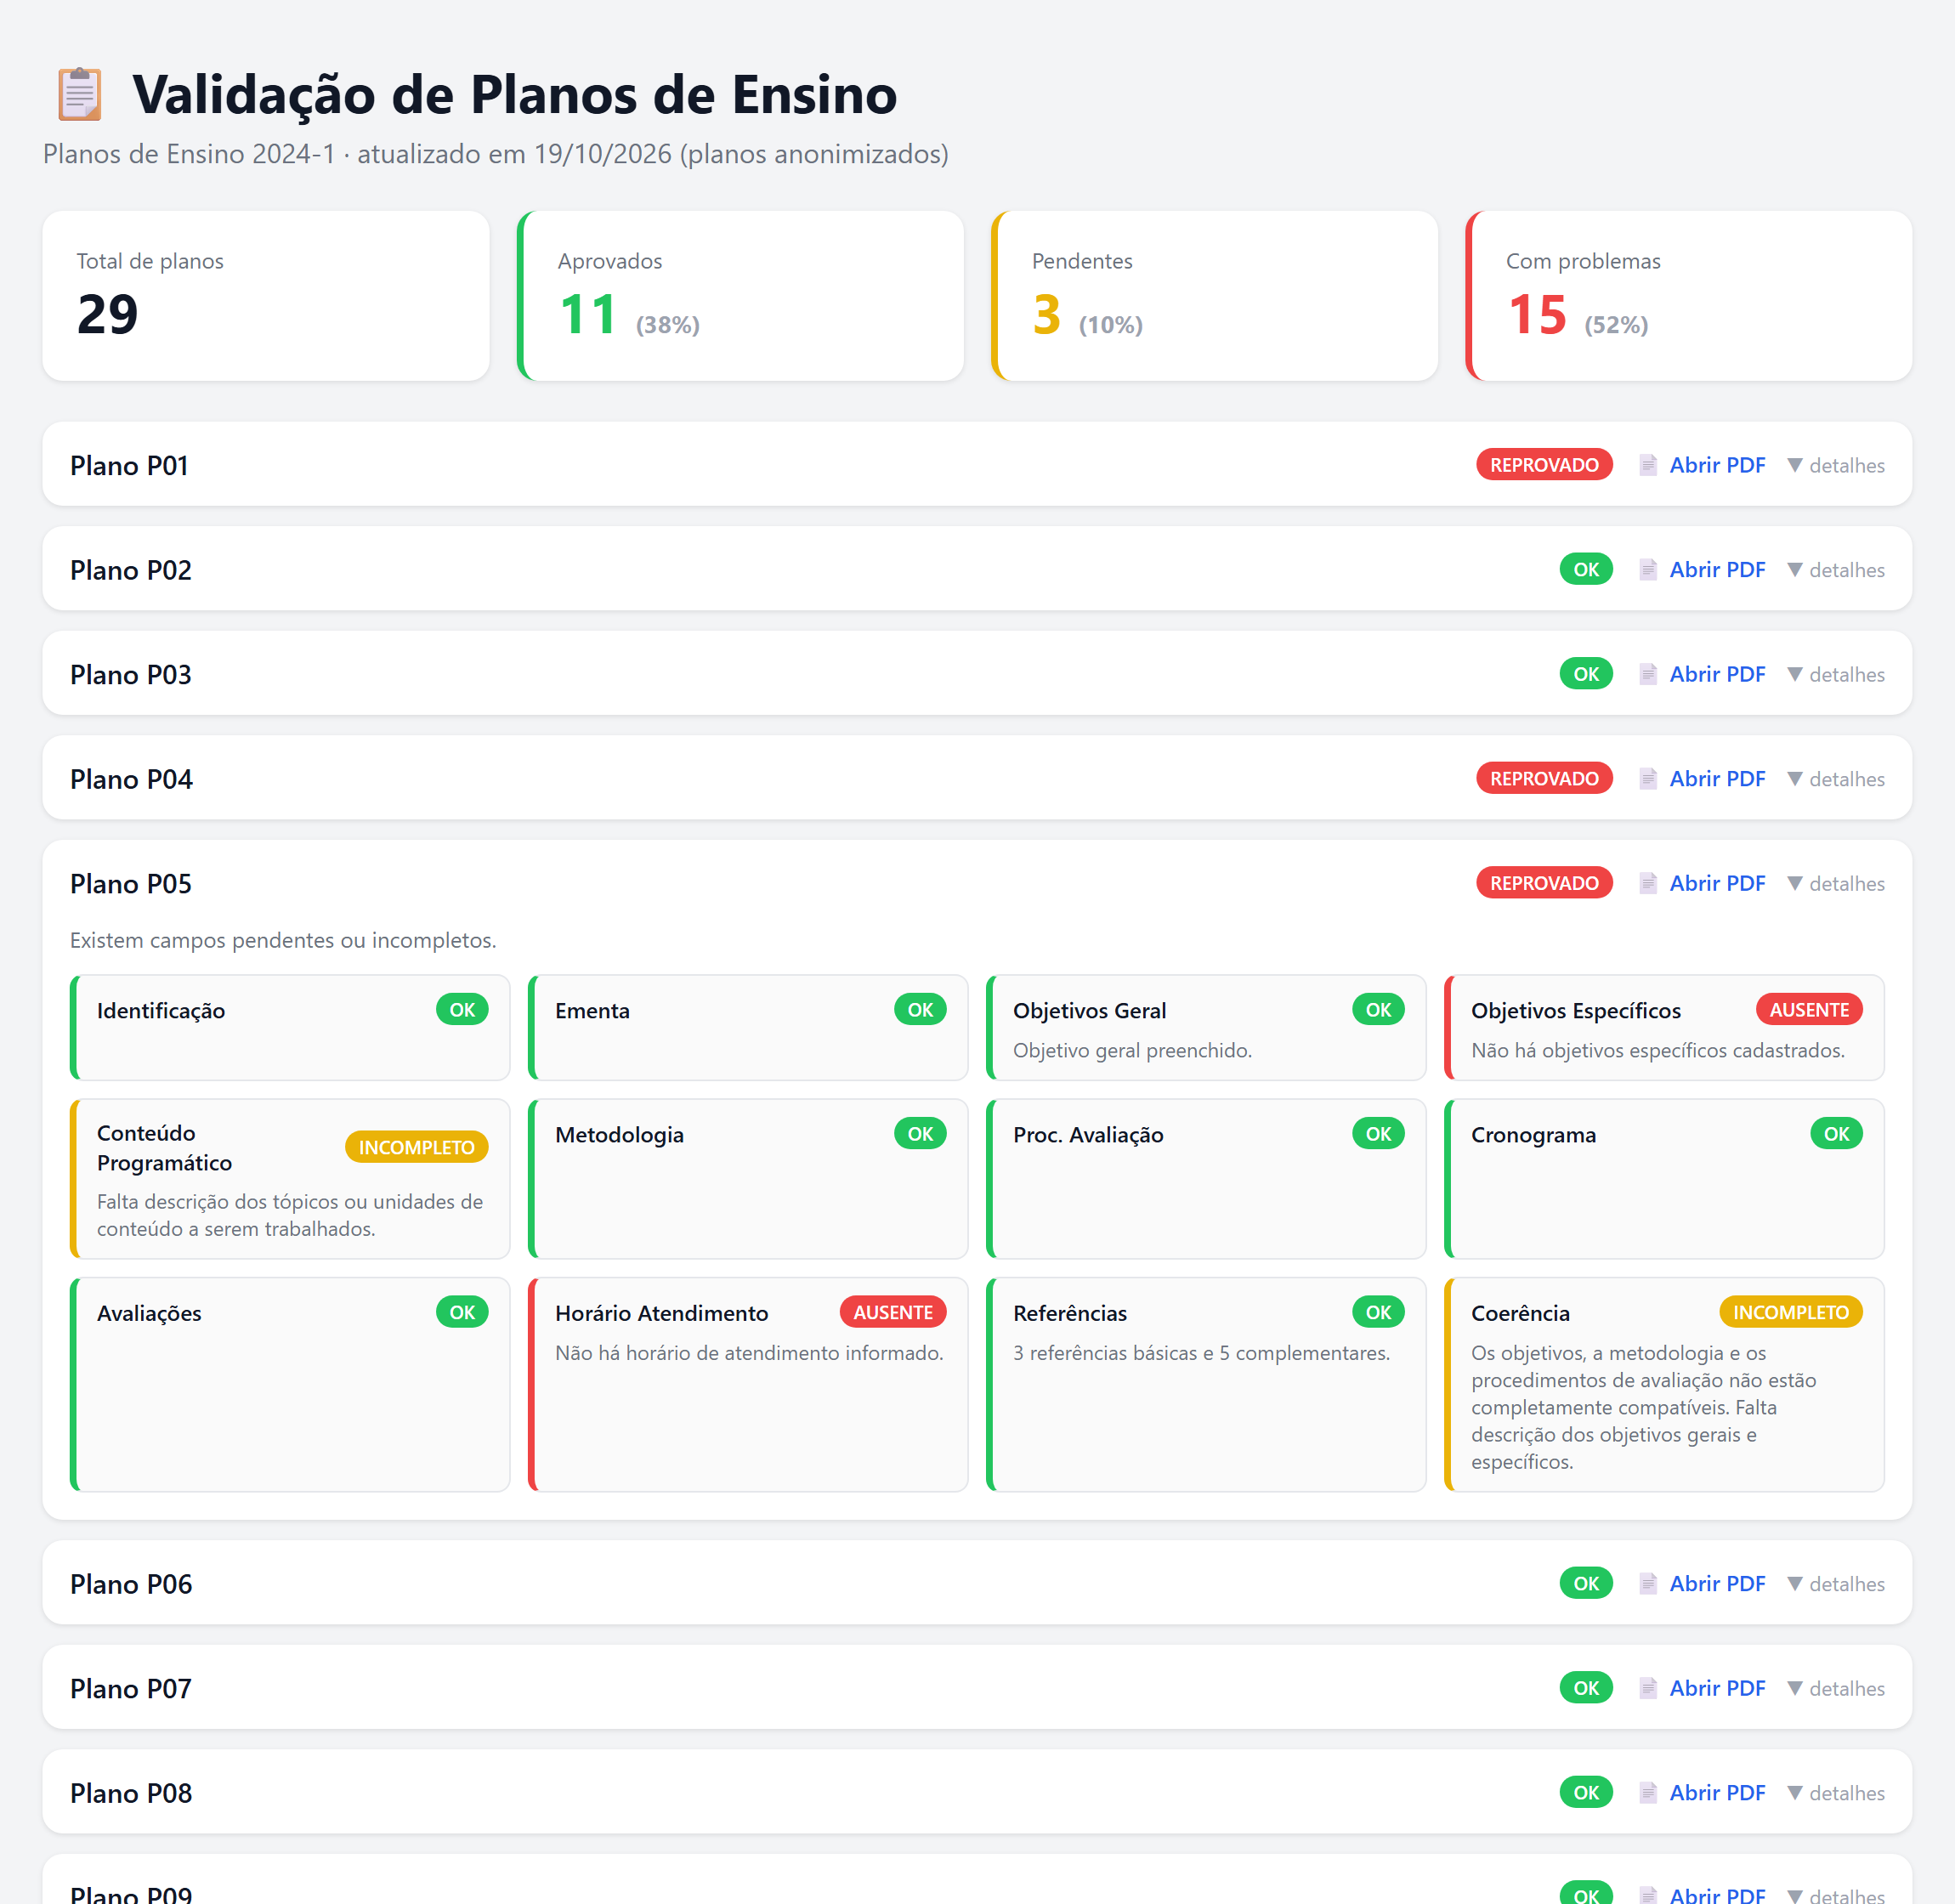
\includegraphics[width=0.92\textwidth]{images/dashboard.png}
\legend{Fonte: Elaborado pelo autor (2026). Nomes dos arquivos substituídos por códigos para anonimização.}
\end{figure}

O plano P05, expandido na figura, ilustra o uso pretendido: o avaliador vê imediatamente que faltam o horário de atendimento e os objetivos específicos e que o conteúdo programático está incompleto, e pode abrir o PDF para confirmar. O mesmo exemplo revela também uma limitação discutida na Seção \ref{sec:res-erros}: o objetivo geral aparece como OK, embora o campo contenha apenas o texto provisório ``Não Cadastrado!'' do SIGAA.

\section{Testes}
\label{sec:testes}

Para garantir que cada etapa descrita neste capítulo funcionasse como esperado ao longo das iterações, a estratégia de testes combinou três abordagens. Os testes de execução, feitos a cada alteração de um nó, usaram o modo de execução manual do n8n, que exibe a entrada e a saída de cada nó e permite inspecionar o resultado da extração, da segmentação, do \textit{prompt} e da resposta do modelo para um plano específico. Os testes de regressão, feitos ao fim de cada iteração, consistiram em processar novamente o corpus completo e comparar os resultados com os da execução anterior, verificando se a correção resolvia o problema visado sem introduzir novos erros. Por fim, a avaliação da versão final, segundo o protocolo da Seção \ref{sec:protocolo}, mediu robustez, desempenho e concordância. Os resultados dessas avaliações são apresentados no Capítulo \ref{cap:resultados}.


% AVALIAÇÃO E RESULTADOS
\chapter{AVALIAÇÃO E RESULTADOS}
\label{cap:resultados}

Este capítulo apresenta e discute os resultados obtidos segundo o protocolo da Seção \ref{sec:protocolo}. A Seção \ref{sec:res-robustez} analisa a robustez técnica ao longo das iterações, a Seção \ref{sec:res-desempenho} trata do desempenho computacional, a Seção \ref{sec:res-corpus} apresenta os resultados da validação dos 29 planos, a Seção \ref{sec:res-oraculo} mede a concordância com o oráculo estrutural e a Seção \ref{sec:res-erros} analisa os erros do sistema. A Seção \ref{sec:res-semestres} amplia a avaliação para os 120 planos de quatro semestres, de 2024/1 a 2025/2, e a Seção \ref{sec:res-discussao} discute os resultados em conjunto. Salvo indicação contrária, os números das Seções \ref{sec:res-robustez} a \ref{sec:res-erros} referem-se à execução da versão final sobre os planos de 2024/1, realizada em 19 de outubro de 2026.

\section{Robustez técnica ao longo das iterações}
\label{sec:res-robustez}

A primeira dimensão avaliada é a robustez técnica, pois um sistema que falha ao processar os planos não pode ter seus resultados avaliados nas demais dimensões. A Figura \ref{fig:evolucao} mostra a proporção de planos que receberam o status ERRO em cada data de execução registrada na planilha de resultados. Nas datas com mais de uma execução, como 25/08, o valor agrega todas as execuções do dia.

\begin{figure}[htbp]
\centering
\caption{Proporção de planos com status ERRO por data de execução}
\label{fig:evolucao}
% Dados: aba Validações da planilha (registros por data de execução) e execução de 19/10/2026
\begin{tikzpicture}
\begin{axis}[
  ybar,
  width=14cm, height=6.6cm,
  bar width=16pt,
  ymin=0, ymax=100,
  ylabel={Planos com status ERRO (\%)},
  symbolic x coords={22/05,07/07,10/08,25/08,10/09,15/09,19/10},
  xtick=data,
  xlabel={Data da execução (2026)},
  nodes near coords={\pgfmathprintnumber[fixed,precision=1]{\pgfplotspointmeta}\%},
  nodes near coords style={font=\scriptsize},
  ticklabel style={font=\scriptsize},
  label style={font=\footnotesize},
  enlarge x limits=0.09,
]
\addplot[fill=black!35, draw=black] coordinates {
  (22/05,86.2) (07/07,3.4) (10/08,69.0) (25/08,49.1) (10/09,0) (15/09,17.2) (19/10,0)};
\end{axis}
\end{tikzpicture}

\legend{Fonte: Elaborado pelo autor (2026), a partir da planilha de resultados (348 registros) e da execução de 19/10/2026.}
\end{figure}

A análise das mensagens de erro registradas permitiu identificar quatro causas de falha, resumidas na Tabela \ref{tab:falhas} com as correções correspondentes.

\begin{table}[H]
\centering
\caption{Causas de falha identificadas e correções aplicadas}
\label{tab:falhas}
\footnotesize
\begin{tabular}{@{}L{3.4cm}L{4.7cm}L{6.3cm}@{}}
\toprule
\rowcolor[HTML]{EFEFEF}
\textbf{Sintoma} & \textbf{Causa} & \textbf{Correção} \\ \midrule
Resposta vazia ou JSON truncado (``\textit{Unexpected end of JSON input}'') & Requisições simultâneas sobrecarregavam o servidor de inferência, que interrompia respostas & Processamento em blocos, uma requisição por vez, com até três tentativas \\
JSON malformado (``\textit{Expected ',' or '\}'}'') & O modelo produzia texto fora da sintaxe JSON & Saída estruturada com esquema JSON no parâmetro \texttt{format} \\
Respostas em outro idioma ou com JSON sem relação com o pedido & O \textit{prompt} (cerca de 5.100 \textit{tokens} à época) excedia o contexto padrão de 4.096 \textit{tokens} e era truncado & Definição explícita do contexto (12.288 e, depois, 8.192 \textit{tokens}) e redução do \textit{prompt} \\
Estouro do tempo limite (\textit{timeout}) & Geração lenta, com parte do modelo fora da GPU e queda de desempenho do equipamento & Contexto de 8.192, \textit{FlashAttention} e \textit{KV cache} em 8 bits \\ \bottomrule
\end{tabular}
\legend{Fonte: Elaborado pelo autor (2026).}
\end{table}

A causa mais frequente foi a resposta vazia ou truncada, responsável por todas as falhas de 22/05 e de 10/08 e por 55 das 57 falhas de 25/08. O problema não estava no modelo, mas na forma de chamá-lo: o n8n enviava as requisições de todos os planos quase ao mesmo tempo, e o servidor as enfileirava e interrompia. A solução foi controlar a concorrência no próprio fluxo, com o laço de blocos da Figura \ref{fig:pipeline}. O comportamento intermitente, com poucas falhas em 07/07 e muitas novamente em 10/08, é compatível com uma falha dependente da carga sobre o servidor, e não de planos específicos. As duas falhas de 07/07 foram de outro tipo, JSON malformado, eliminado com a adoção da saída estruturada.

O truncamento do contexto foi o problema mais difícil de diagnosticar, pois não gerava erro: o Ollama descartava silenciosamente a parte do \textit{prompt} que excedia o contexto padrão, e o modelo, sem parte das instruções, respondia em outro idioma ou produzia um JSON sem relação com o pedido. O episódio ilustra uma característica dos sistemas com LLMs: falhas de configuração podem se manifestar como respostas plausíveis e incorretas, e não como erros explícitos, o que reforça a importância do registro detalhado das execuções defendido pelas práticas de MLOps \cite{Kreuzberger2023}.

Na execução de 15/09, cinco planos falharam por estouro do tempo limite, então de 600 segundos. Os metadados do Ollama mostram que a velocidade de geração caiu de 18,1 para 5,6 \textit{tokens} por segundo em relação à execução de 10/09, com a mesma configuração de inferência, o que indica uma queda de desempenho do equipamento, como o estrangulamento térmico ou a entrada em modo de economia de energia, e não um problema do fluxo. A otimização de memória da iteração de outubro, discutida na próxima seção, e o tempo limite menor, de 180 segundos, com retentativas, tornaram o sistema menos sensível a essas variações. Na execução final, nenhum dos 29 planos falhou.

\section{Desempenho computacional}
\label{sec:res-desempenho}

Eliminadas as falhas técnicas, a questão seguinte é se o sistema processa o lote em tempo compatível com o uso real. A Tabela \ref{tab:desempenho} resume os metadados de inferência da execução final. Cada plano gerou, em média, um \textit{prompt} de 3.248 \textit{tokens} e uma resposta de 274 \textit{tokens}. A leitura do \textit{prompt} levou em média 1,6 segundo e a geração da resposta, 9,9 segundos, totalizando 11,5 segundos de inferência por plano. A velocidade média de geração foi de 27,6 \textit{tokens} por segundo. O lote completo de 29 planos, incluindo a listagem e o \textit{download} dos arquivos, a extração, as chamadas ao modelo e a gravação na planilha, foi processado em 8 minutos e 54 segundos, abaixo do limite de 30 minutos estabelecido no RNF03. Essa execução usou a versão com Google Drive e Google Sheets; na versão final, com pastas locais, a leitura dos arquivos e a gravação dos resultados deixam de passar pela rede, e o tempo total continua dominado pela inferência, que respondeu por cerca de 5,6 dos 8,9 minutos.

\begin{table}[H]
\centering
\caption{Estatísticas de inferência por plano na execução final (n = 29)}
\label{tab:desempenho}
\footnotesize
\begin{tabular}{@{}lrrrrr@{}}
\toprule
\rowcolor[HTML]{EFEFEF}
\textbf{Medida} & \textbf{Mínimo} & \textbf{Máximo} & \textbf{Média} & \textbf{Mediana} & \textbf{Desvio-padrão} \\ \midrule
Páginas do PDF & 3 & 5 & 3,4 & 3 & 0,6 \\
Caracteres extraídos & 4.520 & 11.436 & 7.048 & 6.770 & 1.700 \\
\textit{Tokens} do \textit{prompt} & 2.481 & 4.522 & 3.248 & 3.120 & 558 \\
\textit{Tokens} da resposta & 250 & 347 & 274 & 269 & 18 \\
Tempo de leitura do \textit{prompt} (s) & 0,8 & 11,3 & 1,6 & 1,2 & 1,9 \\
Tempo de geração (s) & 8,9 & 12,3 & 9,9 & 9,8 & 0,6 \\ \bottomrule
\end{tabular}
\legend{Fonte: Elaborado pelo autor (2026), a partir dos metadados do Ollama.}
\end{table}

O tamanho da resposta variou pouco, pois o esquema JSON fixa sua estrutura, e o tempo de geração acompanhou essa estabilidade, com desvio-padrão de apenas 0,6 segundo. O tempo de leitura do \textit{prompt} teve um valor atípico de 11,3 segundos em um dos planos; nos demais, ficou entre 0,8 e 1,9 segundo.

A Figura \ref{fig:desempenho} compara a velocidade de geração em três execuções sobre o mesmo corpus. Entre 10/09 e 19/10, a velocidade passou de 18,1 para 27,6 \textit{tokens} por segundo, um ganho de 52\%, e o tempo total do lote caiu de 46 minutos para menos de 9 minutos. O ganho decorre da combinação de três mudanças na iteração de outubro: a redução do contexto de 12.288 para 8.192 \textit{tokens}, viabilizada pela segmentação mais precisa, que eliminou trechos desnecessários do \textit{prompt}; o \textit{FlashAttention}; e a quantização do \textit{KV cache} em 8 bits. Juntas, essas mudanças reduziram a memória ocupada pelo contexto; na configuração final, o Ollama reportou 92\% do modelo alocado na GPU de 6 GB, com o restante na CPU. A execução de 15/09 é mostrada como referência do efeito da degradação do equipamento discutida na seção anterior.

\begin{figure}[htbp]
\centering
\caption{Velocidade de geração por configuração}
\label{fig:desempenho}
% Dados: metadados das respostas do Ollama nas execuções de 10/09, 15/09 e 19/10/2026 (29 planos cada)
\begin{tikzpicture}
\begin{axis}[
  ybar,
  width=12cm, height=6.4cm,
  bar width=22pt,
  ymin=0, ymax=34,
  ylabel={\textit{Tokens} gerados por segundo},
  symbolic x coords={10/09,15/09,19/10},
  xtick=data,
  xticklabels={{10/09 (contexto 12.288)},{15/09 (degradada)},{19/10 (otimizada)}},
  nodes near coords={\pgfmathprintnumber[fixed,precision=1]{\pgfplotspointmeta}},
  nodes near coords style={font=\scriptsize},
  ticklabel style={font=\scriptsize},
  label style={font=\footnotesize},
  enlarge x limits=0.3,
]
\addplot[fill=black!35, draw=black] coordinates {(10/09,18.1) (15/09,5.6) (19/10,27.6)};
\end{axis}
\end{tikzpicture}

\legend{Fonte: Elaborado pelo autor (2026), a partir dos metadados do Ollama.}
\end{figure}

Extrapolando a média de 11,5 segundos de inferência por plano, a validação dos planos de todos os cursos de um campus, na casa das centenas por semestre, levaria menos de uma hora no mesmo equipamento, executada de madrugada pelo agendamento diário. O desempenho obtido é, portanto, compatível com o uso real, sem custo por requisição e sem envio dos documentos a serviços externos.

\section{Resultados da validação do corpus}
\label{sec:res-corpus}

Com o sistema estável e com desempenho adequado, esta seção apresenta o que ele apontou sobre os planos. Na execução final, 11 planos (37,9\%) foram considerados conformes (OK), 3 (10,3\%) pendentes e 15 (51,7\%) reprovados. A Figura \ref{fig:criterios} detalha o resultado por critério.

\begin{figure}[htbp]
\centering
\caption{Resultado por critério na execução final (29 planos)}
\label{fig:criterios}
% Dados: dados/validacoes_2026-10-19.csv (execução de 19/10/2026, 29 planos)
\begin{tikzpicture}
\begin{axis}[
  xbar stacked,
  width=13.5cm, height=9.2cm,
  bar width=9pt,
  xmin=0, xmax=29,
  xtick={0,5,10,15,20,25,29},
  xlabel={Número de planos},
  ytick=data,
  yticklabels={Identificação,Ementa,Objetivo geral,Objetivos específicos,Conteúdo programático,Metodologia,Proc. de avaliação,Cronograma,Avaliações,Horário de atendimento,Referências,Coerência},
  y dir=reverse,
  ticklabel style={font=\scriptsize},
  label style={font=\footnotesize},
  legend style={at={(0.5,-0.13)}, anchor=north, legend columns=3, font=\scriptsize, draw=none},
  nodes near coords={\pgfmathprintnumber{\pgfplotspointmeta}},
  nodes near coords style={font=\tiny},
  point meta=explicit symbolic,
  enlarge y limits=0.05,
]
\addplot[fill=black!15, draw=black] coordinates {
  (29,1) [29] (28,2) [28] (29,3) [29] (26,4) [26] (28,5) [28] (29,6) [29]
  (29,7) [29] (29,8) [29] (29,9) [29] (13,10) [13] (24,11) [24] (28,12) [28]};
\addplot[fill=black!45, draw=black] coordinates {
  (0,1) [] (1,2) [1] (0,3) [] (2,4) [2] (1,5) [1] (0,6) []
  (0,7) [] (0,8) [] (0,9) [] (1,10) [1] (5,11) [5] (1,12) [1]};
\addplot[fill=black!85, draw=black, nodes near coords style={font=\tiny, text=white}] coordinates {
  (0,1) [] (0,2) [] (0,3) [] (1,4) [1] (0,5) [] (0,6) []
  (0,7) [] (0,8) [] (0,9) [] (15,10) [15] (0,11) [] (0,12) []};
\legend{OK, INCOMPLETO, AUSENTE}
\end{axis}
\end{tikzpicture}

\legend{Fonte: Elaborado pelo autor (2026).}
\end{figure}

Seis critérios foram considerados conformes em todos os planos: identificação, objetivo geral, metodologia, procedimentos de avaliação, cronograma e avaliações. O resultado é esperado para identificação e cronograma, cuja estrutura é gerada pelo próprio SIGAA, e indica que os docentes descrevem de forma consistente a metodologia e os instrumentos de avaliação.

O critério com mais não conformidades foi o horário de atendimento, ausente em 15 planos e incompleto em um. Todos os 15 planos reprovados têm o horário de atendimento ausente, e em 9 deles essa é a única não conformidade. O dado é relevante para a gestão do curso: trata-se de uma informação de interesse direto dos estudantes, de preenchimento simples, cuja ausência em mais da metade dos planos dificilmente seria percebida sem uma verificação sistemática.

O segundo critério mais apontado foi o de referências, incompleto em 5 planos. Em quatro deles faltavam referências complementares: três planos tinham 4 e um não tinha nenhuma das 5 exigidas. No quinto, a proporção estava invertida, com 5 referências básicas e apenas 3 complementares. Os demais apontamentos foram pontuais: objetivos específicos em três planos, e ementa, conteúdo programático e coerência em um plano cada.

\section{Concordância com o oráculo estrutural}
\label{sec:res-oraculo}

Os resultados da seção anterior só são úteis se os apontamentos estiverem corretos. O critério de horário de atendimento, o mais apontado, é também o único que pode ser conferido por uma referência independente do modelo. Para esse critério, o oráculo estrutural descrito na Seção \ref{sec:protocolo} identificou 15 planos com o campo vazio e 14 com conteúdo. A Tabela \ref{tab:confusao} apresenta a matriz de confusão do sistema em relação a esse oráculo, considerando como positivo o plano não conforme, isto é, com status INCOMPLETO ou AUSENTE.

\begin{table}[H]
\centering
\caption{Matriz de confusão do critério horário de atendimento}
\label{tab:confusao}
\footnotesize
\begin{tabular}{@{}lccc@{}}
\toprule
\rowcolor[HTML]{EFEFEF}
 & \textbf{Sistema: não conforme} & \textbf{Sistema: conforme} & \textbf{Total} \\ \midrule
\textbf{Oráculo: campo vazio} & 15 (VP) & 0 (FN) & 15 \\
\textbf{Oráculo: campo preenchido} & 1 (FP) & 13 (VN) & 14 \\
\textbf{Total} & 16 & 13 & 29 \\ \bottomrule
\end{tabular}
\legend{Fonte: Elaborado pelo autor (2026).}
\end{table}

O sistema detectou todos os 15 campos vazios, o que corresponde a um \textit{recall} de 100\%, e apontou um único plano cujo campo estava preenchido, resultando em precisão de 93,8\%, $F_1$ de 0,968 e acurácia de 96,6\%. O Kappa de Cohen foi de 0,931, o que corresponde a concordância quase perfeita na escala de \citeonline{Landis1977}.

O único falso positivo em relação ao oráculo, o plano P19, merece atenção. Seu campo contém a frase ``conforme horário disponibilizado publicamente'', que não informa dia nem horário. Pela regra do critério (Tabela \ref{tab:criterios}), o plano é de fato não conforme, de modo que o apontamento está correto quanto à conformidade, e a divergência decorre da limitação do oráculo, que apenas verifica se o campo está vazio. O erro do modelo está na categoria: deveria ter atribuído INCOMPLETO, pois há conteúdo relacionado, mas atribuiu AUSENTE, contrariando a instrução explícita do \textit{prompt}. Considerando a regra do critério, e não apenas o oráculo estrutural, o sistema acertou a conformidade dos 29 planos e errou a categoria em dois: o P19, como descrito, e o P21, que tem o campo vazio e recebeu INCOMPLETO em vez de AUSENTE.

\section{Análise de erros}
\label{sec:res-erros}

Para os demais critérios, que não têm oráculo estrutural, a correção dos apontamentos foi verificada manualmente. Todos os apontamentos da execução final, além dos de horário de atendimento, foram confrontados com o texto extraído dos PDFs. A Tabela \ref{tab:erros} apresenta o resultado dessa verificação.

\begin{table}[H]
\centering
\caption{Verificação dos apontamentos da execução final (exceto horário de atendimento)}
\label{tab:erros}
\footnotesize
\begin{tabular}{@{}L{1.1cm}L{2.8cm}L{2.4cm}L{4.3cm}L{3.6cm}@{}}
\toprule
\rowcolor[HTML]{EFEFEF}
\textbf{Plano} & \textbf{Critério} & \textbf{Sistema} & \textbf{Conteúdo no PDF} & \textbf{Avaliação} \\ \midrule
P05 & Objetivos específicos & AUSENTE & ``Objetivos: Não Cadastrado!'' & Correto \\
P05 & Conteúdo programático & INCOMPLETO & ``Não Cadastrado!'' & Não conformidade correta; categoria deveria ser AUSENTE \\
P05 & Coerência & INCOMPLETO & Sem objetivos para comparar & Correto \\
P05 & Objetivo geral & OK & ``Não Cadastrado!'' & Falso negativo \\
P20, P21 & Objetivos específicos & INCOMPLETO & Objetivo em parágrafo único, sem objetivos específicos & Não conformidade correta \\
P27 & Ementa & INCOMPLETO & ``A cadastrar'' & Não conformidade correta; categoria deveria ser AUSENTE \\
P11, P23, P25, P28, P29 & Referências & INCOMPLETO & Contagens conferidas no texto & Correto \\ \bottomrule
\end{tabular}
\legend{Fonte: Elaborado pelo autor (2026).}
\end{table}

Todos os 11 apontamentos verificados correspondem a não conformidades reais. Em dois deles, porém, a categoria atribuída foi INCOMPLETO quando o campo continha apenas um texto provisório do SIGAA, situação que deveria ser classificada como AUSENTE. Esse padrão, somado aos dois erros de categoria do horário de atendimento, mostra que o modelo distingue bem a presença de um problema, mas é menos confiável na escolha entre INCOMPLETO e AUSENTE. O caso dos planos P20 e P21, duas turmas do mesmo componente com o campo de horário igualmente vazio, que receberam AUSENTE e INCOMPLETO respectivamente, mostra que essa escolha pode variar mesmo com temperatura 0,1, quando outras partes do \textit{prompt}, como o cronograma, diferem. Como a categoria determina se o plano é REPROVADO ou PENDENTE, essa instabilidade afeta o status geral: o P21 foi classificado como PENDENTE, enquanto o P20, praticamente idêntico, foi REPROVADO.

Foi identificado um falso negativo: o objetivo geral do plano P05 foi considerado OK, embora contivesse apenas o texto provisório ``Não Cadastrado!''. O erro não é do modelo, mas da regra determinística RN04, que considera conforme qualquer texto preenchido. Uma busca por textos provisórios em todo o corpus confirmou que esse foi o único caso em que um texto provisório foi aceito como conteúdo válido; nos outros dois (conteúdo programático do P05 e ementa do P27), o modelo apontou corretamente a não conformidade.

Por fim, a análise revelou um problema de consistência na observação geral, o resumo em uma frase produzido pelo modelo. Em 18 dos 24 planos cujo critério de referências foi considerado conforme, a observação geral mencionava algum problema com as referências, como ``faltam referências básicas''. A contradição ocorre porque a observação geral é escrita pelo modelo antes da aplicação das regras determinísticas, e o modelo, mesmo recebendo a contagem verificada, tende a comentar as referências de forma equivocada. Embora não altere nenhum status, a contradição aparece no \textit{dashboard} e pode confundir o avaliador. A correção indicada é gerar a observação geral por código, a partir dos status finais dos critérios.

\section{Ampliação para quatro semestres}
\label{sec:res-semestres}

As seções anteriores avaliaram o sistema em profundidade sobre os planos de 2024/1. Para verificar se o comportamento se mantém em outros semestres e observar a evolução da conformidade dos planos ao longo do tempo, a versão final, já com armazenamento local, foi executada em 4 de novembro de 2026 sobre os planos dos semestres 2024/1, 2024/2, 2025/1 e 2025/2, disponibilizados pelo orientador em uma pasta compartilhada. A pasta continha 126 arquivos. Seis deles, de 2024/2 a 2025/2, são documentos digitalizados, sem camada de texto, e não puderam ser processados, pois o sistema não realiza reconhecimento óptico de caracteres. Os 120 restantes seguem o modelo do SIGAA e foram todos processados. Os planos foram identificados por códigos de S1-P01 a S4-P28, em que S1 a S4 indicam o semestre, e os resultados anonimizados estão no arquivo \texttt{dados/validacoes\_2026-11-04.csv} do repositório.

\subsection{Resultados por semestre}

A Figura \ref{fig:semestres} apresenta o status geral dos planos em cada semestre. No conjunto, 36 planos (30,0\%) foram considerados conformes, 21 (17,5\%) pendentes e 63 (52,5\%) reprovados. A proporção de planos reprovados variou entre 41,2\%, em 2024/2, e 65,5\%, em 2025/1.

\begin{figure}[htbp]
\centering
\caption{Status geral dos planos por semestre}
\label{fig:semestres}
% Dados: dados/validacoes_2026-11-04.csv (execução de 04/11/2026, 120 planos)
\begin{tikzpicture}
\begin{axis}[
  ybar stacked,
  width=13cm, height=7cm,
  bar width=30pt,
  ymin=0, ymax=36,
  ylabel={Número de planos},
  symbolic x coords={2024/1,2024/2,2025/1,2025/2},
  xtick=data,
  xticklabels={{2024/1 (n = 29)},{2024/2 (n = 34)},{2025/1 (n = 29)},{2025/2 (n = 28)}},
  nodes near coords={\pgfmathprintnumber{\pgfplotspointmeta}},
  nodes near coords style={font=\scriptsize},
  ticklabel style={font=\scriptsize},
  label style={font=\footnotesize},
  legend style={at={(0.5,-0.15)}, anchor=north, legend columns=3, font=\scriptsize, draw=none},
  enlarge x limits=0.2,
]
\addplot[fill=black!15, draw=black] coordinates {(2024/1,11) (2024/2,12) (2025/1,5) (2025/2,8)};
\addplot[fill=black!45, draw=black] coordinates {(2024/1,4) (2024/2,8) (2025/1,5) (2025/2,4)};
\addplot[fill=black!85, draw=black, nodes near coords style={font=\scriptsize, text=white}] coordinates {(2024/1,14) (2024/2,14) (2025/1,19) (2025/2,16)};
\legend{OK, PENDENTE, REPROVADO}
\end{axis}
\end{tikzpicture}

\legend{Fonte: Elaborado pelo autor (2026), a partir da execução de 04/11/2026.}
\end{figure}

O padrão observado em 2024/1 se repete nos demais semestres: o horário de atendimento é, de longe, o critério com mais apontamentos, não conforme em 69 dos 120 planos (57,5\%), seguido pelas referências, incompletas em 17 planos, e pelos objetivos específicos, com 16 apontamentos. Em 43 planos, o horário de atendimento é a única não conformidade. Identificação e objetivo geral foram considerados conformes em todos os planos, e metodologia, cronograma e coerência tiveram no máximo três apontamentos cada.

\subsection{Horário de atendimento e referência a páginas externas}

A ampliação revelou uma mudança na forma de preencher o horário de atendimento. Em 2024/1, os planos não conformes tinham, com uma exceção, o campo vazio. A partir de 2024/2, muitos docentes passaram a preenchê-lo apenas com uma referência externa, em geral o endereço da página em que o campus publica os planos de trabalho docente (\texttt{videira.ifc.edu.br/ptd-e-rtd}), sem indicar dia nem horário. A Tabela \ref{tab:horario-semestres} resume essa mudança.

\begin{table}[H]
\centering
\caption{Conteúdo do campo de horário de atendimento nos planos não conformes}
\label{tab:horario-semestres}
\footnotesize
\begin{tabular}{@{}lccccc@{}}
\toprule
\rowcolor[HTML]{EFEFEF}
\textbf{Conteúdo do campo} & \textbf{2024/1} & \textbf{2024/2} & \textbf{2025/1} & \textbf{2025/2} & \textbf{Total} \\ \midrule
Vazio & 15 & 8 & 5 & 7 & 35 \\
Endereço da página de PTD & 0 & 6 & 13 & 10 & 29 \\
Outra referência externa (``conforme horário divulgado'') & 1 & 1 & 3 & 0 & 5 \\ \midrule
\textbf{Total de planos não conformes} & \textbf{16} & \textbf{15} & \textbf{21} & \textbf{17} & \textbf{69} \\ \bottomrule
\end{tabular}
\legend{Fonte: Elaborado pelo autor (2026).}
\end{table}

Essa mudança tem dois efeitos sobre a avaliação. O primeiro é sobre o oráculo estrutural da Seção \ref{sec:res-oraculo}, que considera conforme qualquer campo preenchido. Sobre os 120 planos, o sistema manteve \textit{recall} de 100\%, mas a precisão em relação a esse oráculo caiu para 50,7\% e o Kappa de Cohen para 0,47, porque os 34 campos com referência externa contam como falsos positivos. Conferidos um a um, porém, nenhum desses 34 campos informa dia ou horário, de modo que todos são não conformes pela regra do critério (Tabela \ref{tab:criterios}), e todos os 51 planos considerados conformes informam dia ou horário explicitamente. Pela regra, o sistema acertou a conformidade do horário de atendimento nos 120 planos. Repete-se, contudo, o erro de categoria já observado no P19: em 33 dos 34 campos com referência externa, o modelo atribuiu AUSENTE, quando deveria atribuir INCOMPLETO. O episódio mostra que um oráculo estrutural válido em um semestre pode deixar de sê-lo quando a prática de preenchimento muda, e reforça a necessidade da anotação humana prevista no protocolo.

O segundo efeito é normativo. A Organização Didática exige que o plano informe o horário de atendimento \cite{ifc2022}, mas não diz se uma referência à página de PTD do campus atende a essa exigência. A decisão cabe à coordenação e ao NDE, e o impacto é grande: se a referência externa fosse aceita, o número de planos reprovados nos quatro semestres cairia de 63 para 30, e o de planos conformes subiria de 36 para 63. A regra do critério pode ser ajustada no \textit{prompt} em qualquer dos dois sentidos, mas a escolha é institucional, e não técnica.

\subsection{Reprodutibilidade e desempenho}

Os 29 planos de 2024/1 foram processados novamente nessa execução, com a mesma configuração de inferência, o que permitiu medir a reprodutibilidade dos resultados. Das 377 classificações (12 critérios e o status geral de cada plano), 374 (99,2\%) foram idênticas às da execução de 19 de outubro. As três diferenças envolvem, mais uma vez, a escolha entre INCOMPLETO e AUSENTE e mudaram o status geral de um plano, o P20, de REPROVADO para PENDENTE.

O desempenho, por outro lado, foi bem inferior ao da Seção \ref{sec:res-desempenho}. Com outros programas abertos ocupando parte da memória da GPU, o Ollama alocou 14\% do modelo na CPU, contra 8\% na execução de outubro, e cada plano passou a levar de 30 a 60 segundos de inferência. Essa lentidão expôs uma fragilidade do fluxo: o nó de requisição envia um plano por segundo dentro de cada bloco de 10, sem aguardar a resposta anterior, e o servidor de inferência os enfileira. Com 11,5 segundos por plano, o último do bloco termina antes do tempo limite de 180 segundos; com 30 segundos ou mais, não termina. Na primeira tentativa, 55 planos receberam o status ERRO por estouro do tempo limite. Esses planos foram reprocessados com o tempo limite ampliado para 900 segundos, e todos foram avaliados. O episódio mostra que o controle de concorrência descrito na Tabela \ref{tab:falhas} depende do desempenho do equipamento, e que o fluxo deveria aguardar cada resposta antes de enviar o plano seguinte, o que é indicado como trabalho futuro.

\section{Discussão}
\label{sec:res-discussao}

As seções anteriores analisaram cada dimensão da avaliação separadamente. Considerados em conjunto, os resultados permitem responder ao problema de pesquisa sob três aspectos. Quanto à viabilidade técnica, o sistema processou o corpus completo sem falhas, em menos de 9 minutos, em um computador portátil com GPU de 6 GB e sem custos por requisição. A evolução das iterações mostra, porém, que essa robustez não veio do modelo, mas da engenharia em torno dele: controle de concorrência, saída estruturada, dimensionamento do contexto e registro detalhado das execuções. Esse resultado é coerente com a visão de \citeonline{Kreuzberger2023} de que sistemas com componentes de aprendizado de máquina dependem tanto da infraestrutura e da operação quanto do modelo.

Quanto à qualidade da triagem, o sistema não deixou de apontar nenhuma das não conformidades verificáveis por oráculo e todos os seus apontamentos verificados correspondiam a problemas reais, com um único falso negativo identificado, causado por uma regra determinística e não pelo modelo. A principal fragilidade está na distinção entre INCOMPLETO e AUSENTE. Para uma ferramenta de triagem, cujo objetivo é dirigir a atenção do avaliador, a detecção do problema é mais importante que sua categoria, mas a categoria afeta o status geral e, portanto, a priorização dos planos. Esses resultados estão alinhados com a literatura sobre LLMs como avaliadores, que relata boa concordância com humanos acompanhada de vieses e inconsistências que precisam ser controlados \cite{Zheng2023, Chang2024}.

Quanto à divisão de trabalho entre regras e modelo, os resultados confirmam a decisão de projeto. Os critérios mais objetivos, como a contagem de referências, tornaram-se exatos quando passaram a ser verificados por código, enquanto, nos critérios interpretativos, todos os apontamentos feitos pelo modelo foram confirmados na verificação, inclusive o de coerência. Ao mesmo tempo, o falso negativo do P05 mostra que as regras determinísticas também precisam ser validadas: uma regra simples demais (``preenchido é conforme'') introduziu um erro que o modelo, no mesmo plano, não cometeu nos demais campos com texto provisório. A combinação mais robusta, apontada como trabalho futuro, é usar regras para detectar campos vazios ou provisórios, atribuindo-lhes AUSENTE de forma determinística, e reservar o modelo para julgar a qualidade dos campos preenchidos.

Do ponto de vista da gestão do curso, o sistema evidenciou um problema concreto e sistemático, a falta do horário de atendimento em mais da metade dos planos, que se manteve nos quatro semestres analisados e que, a partir de 2024/2, passou a envolver também a substituição do horário por uma referência à página de PTD do campus. O primeiro caso pode ser tratado com uma orientação aos docentes no início do semestre; o segundo exige antes uma definição do NDE sobre o que conta como horário informado. Esse tipo de diagnóstico agregado, difícil de obter em uma conferência manual plano a plano, ilustra o potencial da ferramenta para apoiar ações da coordenação e do NDE, em linha com as aplicações de IA na gestão educacional descritas por \citeonline{Sposato2025}.

É importante delimitar o alcance desses resultados. A concordância foi medida com um oráculo estrutural em um único critério e completada pela verificação dos apontamentos do sistema, o que permite estimar a precisão dos apontamentos, mas não o \textit{recall} nos critérios interpretativos: um plano cuja metodologia fosse inadequada e tivesse sido considerada OK pelo sistema não seria detectado por esse procedimento. A estimativa completa exige a anotação de todos os critérios por avaliadores humanos, conforme o protocolo da Seção \ref{sec:protocolo}. Além disso, a avaliação detalhada foi feita sobre os 29 planos de 2024/1; a ampliação para quatro semestres confirmou a estabilidade do sistema e o padrão de não conformidades, mas segue restrita a um único curso.


%CONCLUSÃO
\chapter{CONCLUSÃO}
\label{cap:conclusao}

Este trabalho investigou de que forma um sistema baseado em modelos de linguagem pode apoiar a validação de planos de ensino, reduzindo o esforço de conferência manual e preservando a aderência às normas do IFC e o controle humano sobre a decisão final. Para responder a essa questão, foi desenvolvido e avaliado um sistema semiautomático que obtém os planos de ensino de uma pasta compartilhada, extrai e segmenta seu texto, avalia doze critérios com um LLM aberto executado localmente, combina essa avaliação com regras determinísticas e apresenta os resultados em um painel \textit{web}.

Os objetivos específicos foram atendidos. Os elementos obrigatórios do plano de ensino foram convertidos em doze critérios com regras explícitas, definidos a partir da Organização Didática do IFC e das orientações do orientador e ajustados ao longo das iterações (objetivo 1). O \textit{pipeline} de automação foi implementado no n8n, com extração e segmentação de texto, saída estruturada por esquema JSON, regras determinísticas e registro rastreável de cada validação (objetivo 2). O \textit{dashboard} permite acompanhar os indicadores do lote, consultar o status e a justificativa de cada critério e abrir o PDF original (objetivo 3). Por fim, o sistema foi avaliado com os 29 planos de ensino do semestre 2024/1 quanto à robustez, ao desempenho e à concordância, e a análise de erros resultou em propostas concretas de aprimoramento (objetivo 4).

Os resultados mostram que a abordagem é viável. Ao longo de cinco iterações, a proporção de planos com falha técnica caiu de 86,2\% para zero, e a versão final processou o lote completo em 8 minutos e 54 segundos, com 11,5 segundos de inferência por plano em uma GPU de 6 GB, sem custos por requisição e sem envio dos documentos a serviços externos. No critério verificável por oráculo estrutural, o sistema alcançou \textit{recall} de 100\%, precisão de 93,8\% e Kappa de Cohen de 0,93, e todos os apontamentos verificados nos demais critérios correspondiam a não conformidades reais. A validação revelou ainda um problema sistemático no curso, a ausência do horário de atendimento em mais da metade dos planos, que dificilmente seria percebido em uma conferência manual plano a plano.

A principal lição do trabalho é que a confiabilidade de um sistema com LLMs depende menos do modelo do que da engenharia em torno dele. As falhas mais graves das primeiras versões, como respostas truncadas, JSON malformado e \textit{prompts} cortados pelo limite de contexto, foram resolvidas com controle de concorrência, saída estruturada e dimensionamento do contexto, e não com a troca do modelo. Da mesma forma, atribuir as verificações exatas a regras determinísticas e os julgamentos interpretativos ao modelo mostrou-se uma divisão de trabalho eficaz, desde que as próprias regras também sejam validadas, como evidenciou o falso negativo causado pela aceitação de um texto provisório do SIGAA.

\section{Limitações}

Os resultados devem ser interpretados à luz de algumas limitações. A primeira é a ausência de uma referência humana completa: a concordância foi medida com um oráculo estrutural em um único critério e complementada pela verificação dos apontamentos do sistema, o que permite avaliar a precisão dos apontamentos, mas não estimar os falsos negativos nos critérios interpretativos. A anotação de todos os critérios por membros do NDE, prevista no protocolo da Seção \ref{sec:protocolo} e para a qual foram preparados os artefatos do Apêndice \ref{ap:analise}, não coube no período deste trabalho. A segunda é o tamanho e a homogeneidade do corpus: 29 planos de um único curso, de um único semestre e de um único sistema de origem. A terceira é a dependência do formato do SIGAA, pois a segmentação se baseia nos rótulos de suas seções e precisaria ser revista caso o modelo do documento mude. A quarta é a instabilidade do modelo na escolha entre INCOMPLETO e AUSENTE, que afeta o status geral de alguns planos. Por fim, não foi realizada uma avaliação com usuários sobre a utilidade percebida do \textit{dashboard} e o impacto real na carga de trabalho da coordenação.

\section{Trabalhos futuros}
\label{sec:futuros}

A partir dos resultados e das limitações, sugerem-se os seguintes trabalhos futuros:

\begin{itemize}
    \item \textbf{Avaliação com o NDE}: executar o protocolo de anotação humana de todos os critérios e calcular, por critério, precisão, \textit{recall}, $F_1$ e Kappa de Cohen, ampliando o corpus para outros semestres e cursos.
    \item \textbf{Detecção determinística de campos vazios e provisórios}: atribuir AUSENTE por regra a seções vazias ou que contenham apenas textos provisórios do SIGAA, como ``Não Cadastrado!'' e ``A cadastrar'', eliminando o falso negativo identificado e a instabilidade entre INCOMPLETO e AUSENTE nesses casos.
    \item \textbf{Observação geral gerada por código}: produzir o resumo de cada plano a partir dos status finais dos critérios, eliminando as contradições observadas.
    \item \textbf{RAG sobre documentos normativos extensos}: incorporar o PPC do curso e as ementas oficiais em uma base vetorial, permitindo verificar, por exemplo, se a ementa e as referências do plano correspondem às aprovadas no PPC.
    \item \textbf{Comparação de modelos}: avaliar modelos maiores ou mais recentes, locais e externos, comparando qualidade, tempo e custo sobre o mesmo corpus.
    \item \textbf{Integração ao fluxo institucional}: notificar automaticamente os docentes sobre os itens pendentes e integrar a validação ao momento de cadastro do plano no SIGAA, antes de sua publicação.
    \item \textbf{Avaliação com usuários}: medir, com coordenadores, membros do NDE e docentes, a utilidade percebida, a clareza das justificativas e o tempo economizado em relação à conferência manual.
\end{itemize}


% ----------------------------------------------------------
% ELEMENTOS PÓS-TEXTUAIS
% ----------------------------------------------------------
\postextual

% ----------------------------------------------------------
% Referências bibliográficas
% ----------------------------------------------------------

\bibliography{referencias}

%Apêndices
\begin{apendicesenv}

\chapter{\textit{Prompt} e esquema JSON enviados ao modelo}
\label{ap:prompt}

Este apêndice reproduz o código do nó \textit{Preparar Prompt} do fluxo de validação, que monta, para cada plano, o \textit{prompt} enviado ao modelo de linguagem, o esquema JSON usado no parâmetro \texttt{format} do Ollama e o \textit{payload} alternativo para a API do Google Gemini. As expressões \texttt{\$\{\ldots\}} são substituídas pelo texto de cada seção do plano no momento da execução.

\lstinputlisting[language=JavaScript]{codigo/preparar_prompt.js}

\chapter{Segmentação do texto e interpretação da resposta}
\label{ap:segmentacao}

O trecho a seguir mostra uma parte do texto extraído de um dos planos do corpus (P05) pelo nó \textit{Extract from File}. Nele se observam as características discutidas no Capítulo \ref{cap:desenvolvimento}: as quebras de linha da diagramação, o campo de horário de atendimento vazio, imediatamente seguido pela seção ``Programa'', e os textos provisórios ``Não Cadastrado!'' do SIGAA.

\begin{lstlisting}[numbers=none]
Horário de Atendimento:
Programa
Objetivos: Não Cadastrado!
Conteúdo Programático: Não Cadastrado!
Cronograma de Aulas - Total de aulas da Turma: 72
Início Fim Descrição
16/02/2024 13/03/2024 Integrais, derivadas parciais e suas aplicações
\end{lstlisting}

O código do nó \textit{Separar Texto por Tópicos}, que segmenta o texto nas seções do plano e conta as referências bibliográficas, é reproduzido a seguir.

\lstinputlisting[language=JavaScript]{codigo/separar_topicos.js}

O código do nó \textit{Parsear Validação}, que interpreta a resposta do modelo, aplica as regras determinísticas e monta o registro gravado na pasta de resultados, é reproduzido a seguir.

\lstinputlisting[language=JavaScript]{codigo/parsear_validacao.js}

\chapter{Artefatos para a análise dos resultados}
\label{ap:analise}

Os dados e \textit{scripts} usados no Capítulo \ref{cap:resultados} acompanham este trabalho no repositório do projeto, na pasta \texttt{tcc-final/dados}:

\begin{itemize}
    \item \texttt{validacoes\_2026-10-19.csv}: resultado anonimizado da execução final, com uma linha por plano, os status dos doze critérios, a contagem de referências, os metadados de inferência e o indicador do oráculo estrutural do horário de atendimento;
    \item \texttt{anotacao\_humana\_modelo.csv}: planilha de anotação com uma linha por par (plano, critério), contendo o status atribuído pelo sistema e colunas em branco para o parecer humano (OK, INCOMPLETO ou AUSENTE) e para comentários;
    \item \texttt{analise.py}: \textit{script} que calcula as estatísticas descritivas, a concordância com o oráculo estrutural e, quando recebe a planilha de anotação preenchida, as métricas da Seção \ref{sec:metricas} por critério e no total.
\end{itemize}

Para executar o protocolo de comparação com o NDE, recomenda-se ocultar a coluna \texttt{sistema} da planilha de anotação antes de distribuí-la aos avaliadores, para que o parecer humano não seja influenciado pela saída do sistema. Após a consolidação dos pareceres, as métricas são obtidas com o comando \texttt{python analise.py anotacao\_humana.csv}. O código do \textit{script} é reproduzido a seguir.

\lstinputlisting[language=Python]{dados/analise.py}

\end{apendicesenv}


%Anexos
% \begin{anexosenv}
\chapter{Título do Anexo A}
\label{anexoA}

Arquivos não confeccionados pelo autor do trabalho.


\end{anexosenv}

%---------------------------------------------------------------------
% INDICE REMISSIVO
%---------------------------------------------------------------------
% \printindex
\end{document}